\documentclass{beamer}


\setbeamertemplate{sections/subsections in toc}[square]
\setbeamertemplate{caption}[numbered]
\setbeamertemplate{footline}[frame number]
\setbeamertemplate{headline}{}
\usepackage{graphicx, tikz, url, animate, tabularx}
\usepackage{caption}
\usepackage[sorting = nyt]{biblatex}
\usepackage{euscript}
\usetikzlibrary{3d, calc}
\newcommand{\euler}[1]{\boldsymbol{\EuScript{#1}}}
\newcommand{\romanL}[1]{\boldsymbol{\mathrm{#1}}}
\addbibresource{bibliography.bib}
\title{Simulation of Quantum Systems using Matrix Product States}
\author{Chase Hodges-Heilmann}
\date{}
\newcommand\blfootnote[1]{%
  \begingroup
  \renewcommand\thefootnote{}\footnote{#1}%
  \addtocounter{footnote}{-1}%
  \endgroup
}


\begin{document}

\maketitle

\begin{frame}{Table of Contents}
    \tableofcontents
\end{frame}




\AtBeginSection[]
{
  \begin{frame}
    \frametitle{Table of Contents}
    \tableofcontents[currentsection]
  \end{frame}
}
Bond Dimension:
\begin{frame}{Tensor Notation}
    An order-$N$ tensor is an $N$-dimensional array. Scalars, vectors, and matrices are special cases of tensors:
    \begin{itemize}
        \item \textbf{Order 0 (scalar)}: $m$
        \item \textbf{Order 1 (vector)}: $\romanL{m}$
        \item \textbf{Order 2 (matrix)}: $\romanL{M}$
        \item \textbf{Order $N > 2$ (tensor)}: $\euler{M}$
    \end{itemize}
    \pause
    Element notation:
    \[
        m_{i_1, i_2, \ldots, i_N} = \euler{M}(i_1, i_2, \ldots, i_N)
    \]

    \blfootnote{\citetitle{Ballard_Kolda_2025}}
\end{frame}

\begin{frame}{Tensor Diagrams}
    Tensor network diagrams represent tensors as nodes with edges (legs) for each index:
    \begin{itemize}
        \item Vector (order 1): One leg
        \item Matrix (order 2): Two legs
        \item Order-3 tensor: Three legs
    \end{itemize}

    \begin{center}
        \begin{tabular}{ccc}
            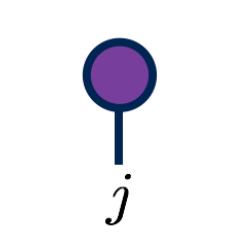
\includegraphics[height=2.5cm]{images/TensorNetwork Images/VectorTensor.png} &
            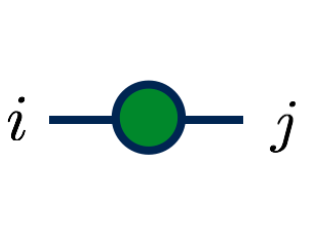
\includegraphics[height=2.5cm]{images/TensorNetwork Images/MatrixTensor.png} &
            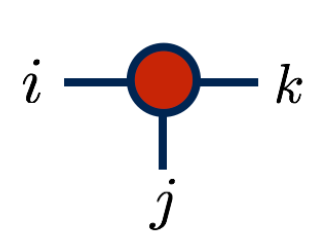
\includegraphics[height=2.5cm]{images/TensorNetwork Images/TensorDiagram_2.png} \\
            Vector $\romanL{v}(i)$ & Matrix $\romanL{M}(i, j)$ & Tensor $\euler{T}(i, j, k)$
        \end{tabular}
    \end{center}

    \blfootnote{\url{https://tensornetwork.org/}}
\end{frame}

\begin{frame}{Tensor Contraction}
    \textbf{Tensor contraction} is a generalization of matrix multiplication, summing over shared indices:

    \begin{itemize}
        \item Examples include:
        \begin{itemize}
            \item Matrix–Vector product\\
                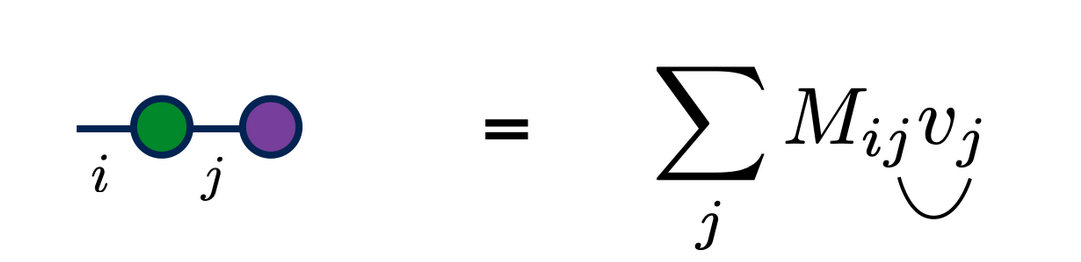
\includegraphics[height=1.25cm]{images/TensorNetwork Images/MatVecContraction.png}
            \item Matrix–Matrix product\\
                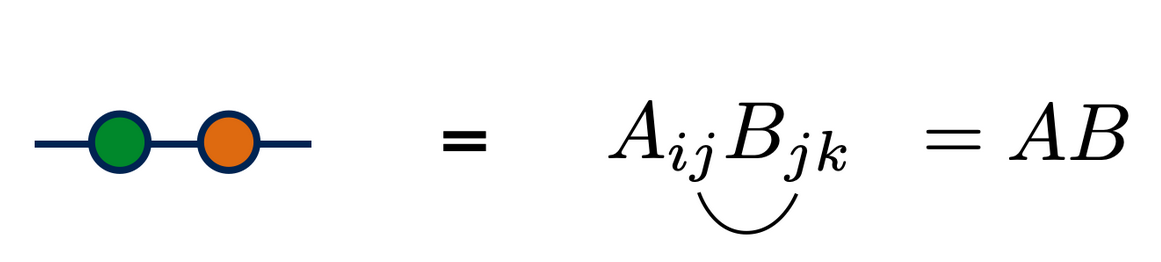
\includegraphics[height=1.25cm]{images/TensorNetwork Images/MatMatContraction.png}
            \item Tensor–Matrix product\\
                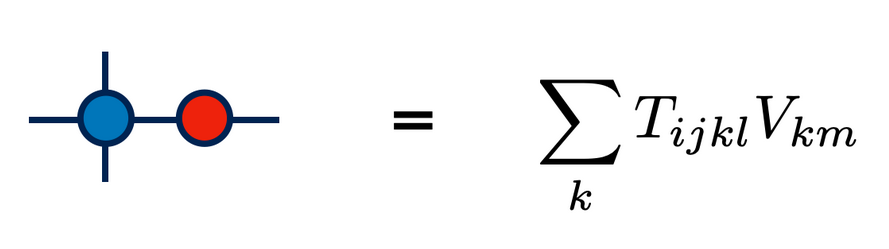
\includegraphics[height=1.25cm]{images/TensorNetwork Images/TensorMatContraction.png}
        \end{itemize}
    \end{itemize}

    \vspace{0.5em}
    \blfootnote{\url{https://tensornetwork.org/}}
\end{frame}

\begin{frame}{Tensor Train/Matrix Product States}
    \small
    A quantum state with $N$ qubits can be written as \begin{equation}
        |\psi\rangle = \sum_{\sigma_1,...,\sigma_N}c_{\sigma_1,...,\sigma_N}|\sigma_1\rangle\otimes...\otimes|\sigma_N\rangle.
    \end{equation}
    \pause
    $c_{\sigma_1,...,\sigma_N}$ is an entry from the $N$ order tensor $\euler{C} \in \mathbb{C}^{\sigma_1 \times \sigma_2 \times ... \times \sigma_N}$. \\
    \pause
    A tensor train (or matrix product state) expresses a high-order tensor $\euler{C}$ as a product of lower-rank tensors:
    \begin{equation}
        \euler{C} = \romanL{M}_1 \cdot \euler{M}_2 \cdot \dots \cdot \euler{M}_{N-1} \cdot \romanL{M}_N
    \end{equation}
    
    \begin{figure}
        \centering
        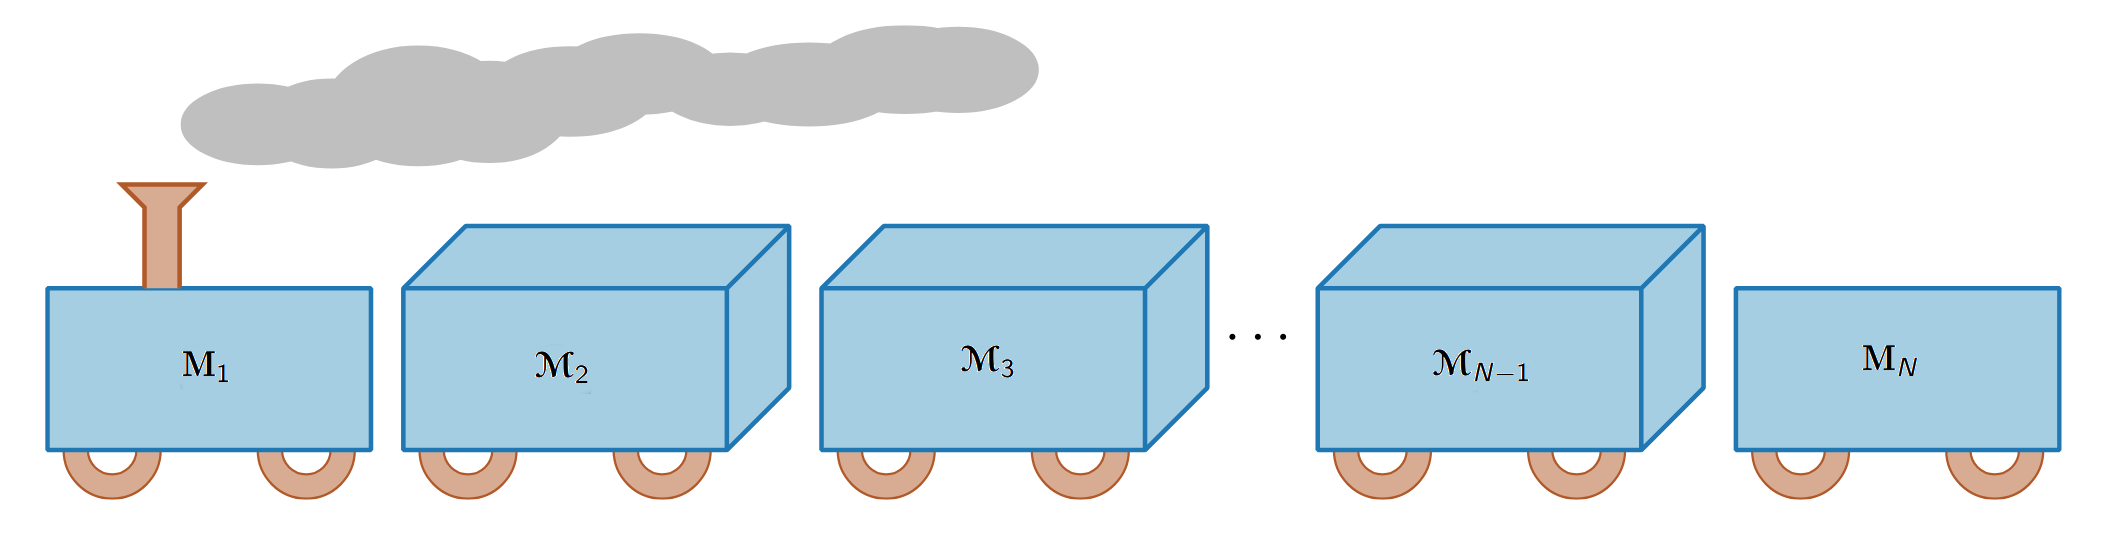
\includegraphics[width=0.90\linewidth]{images/Misc/TensorTrain.png}
        \caption{A Tensor "Train", each train car is called a core.}
        \label{fig:TensorTrain}
    \end{figure}
    \blfootnote{\citetitle{Ballard_Kolda_2025}}
\end{frame}

\begin{frame}{Tensor Train / Matrix Product States}
    \scriptsize
    
    \begin{figure}
        \centering
        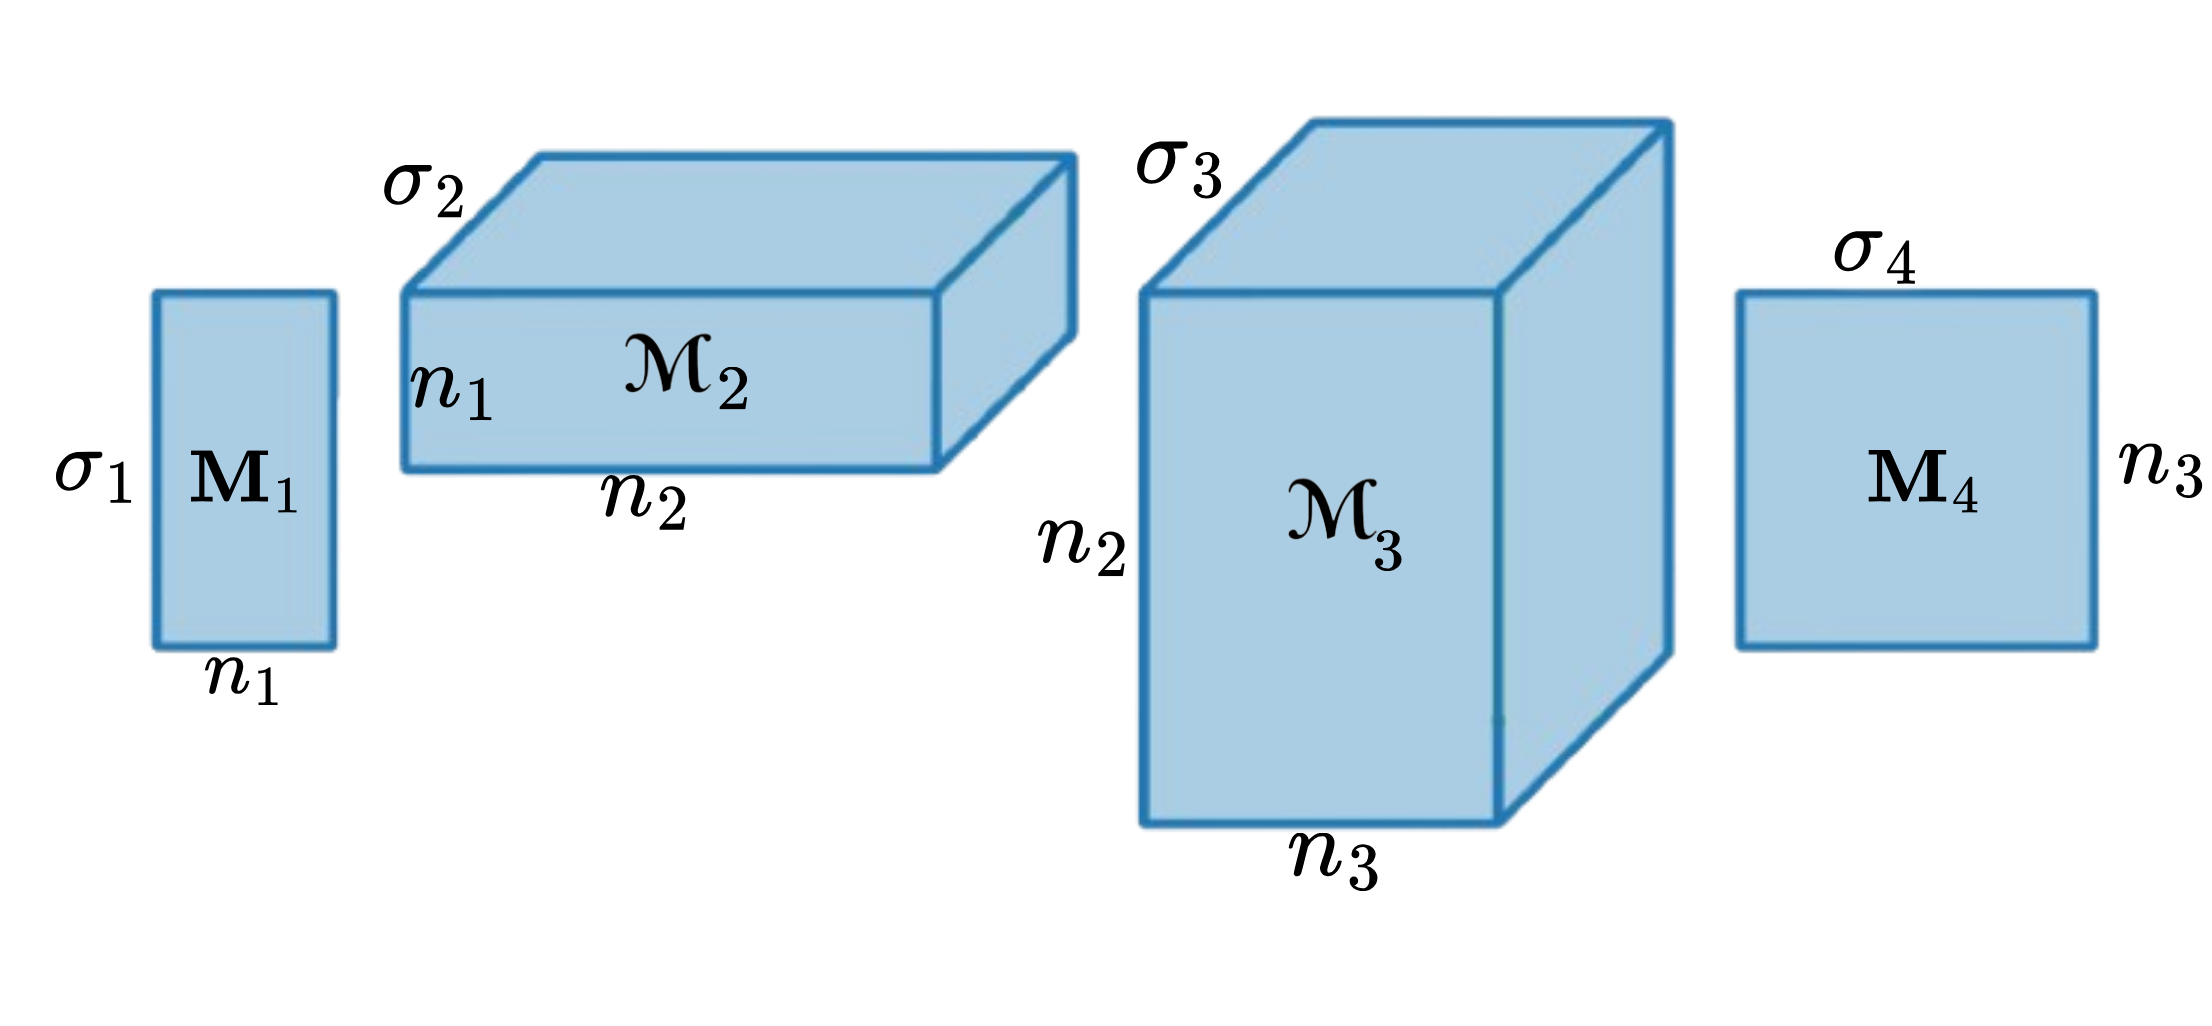
\includegraphics[width = 0.55\linewidth]{images/Misc/MPS_Closer2.png}
        \caption{\scriptsize Dimensions of tensors in 4 site MPS, the $n_i$ dimensions are called bond dimensions.}
        \label{fig:MPS_closer}
    \end{figure}
    \pause
    \begin{figure}
        \centering
        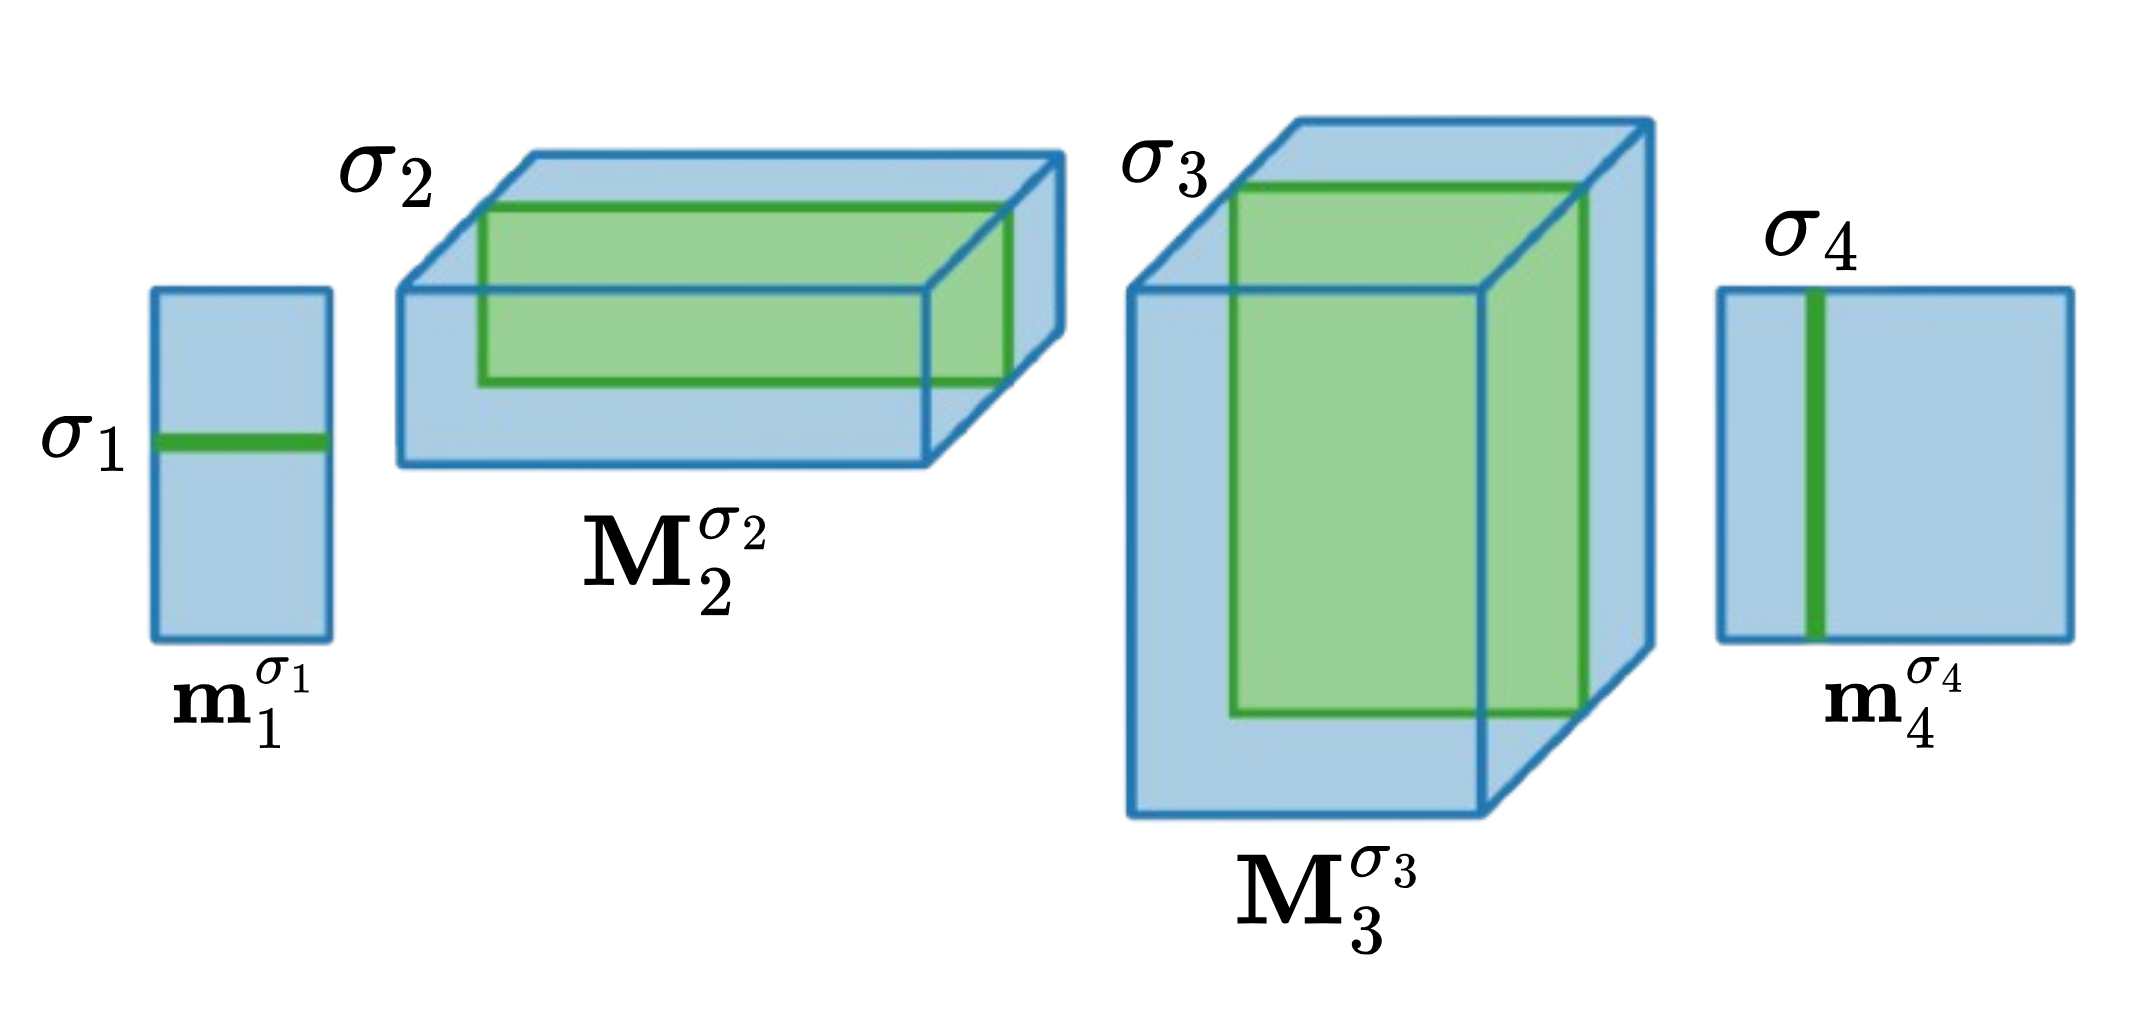
\includegraphics[width=0.55\linewidth]{images/Misc/MPS_element_2.png}
        % \caption{\scriptsize An entry of $\euler{C}(\sigma_1, \ldots, \sigma_N)$ corresponds to multiplying slices of these tensors}
        \label{fig:MPS_Element}
    \end{figure}
    \blfootnote{\citetitle{Ballard_Kolda_2025}}
\end{frame}

\begin{frame}{MPS Diagram}
    
    We can write our quantum state now as 
    \begin{equation}
        |\psi\rangle = \sum_{\sigma_1,...\sigma_N}\romanL{m}_1^{\sigma_1}\romanL{M}_2^{\sigma_2}...\romanL{M}_{N - 1}^{\sigma_{N - 1}}\romanL{m}_N^{\sigma_N}|\sigma_1\rangle \otimes...\otimes|\sigma_N\rangle
    \end{equation}

    \begin{figure}
        \centering
        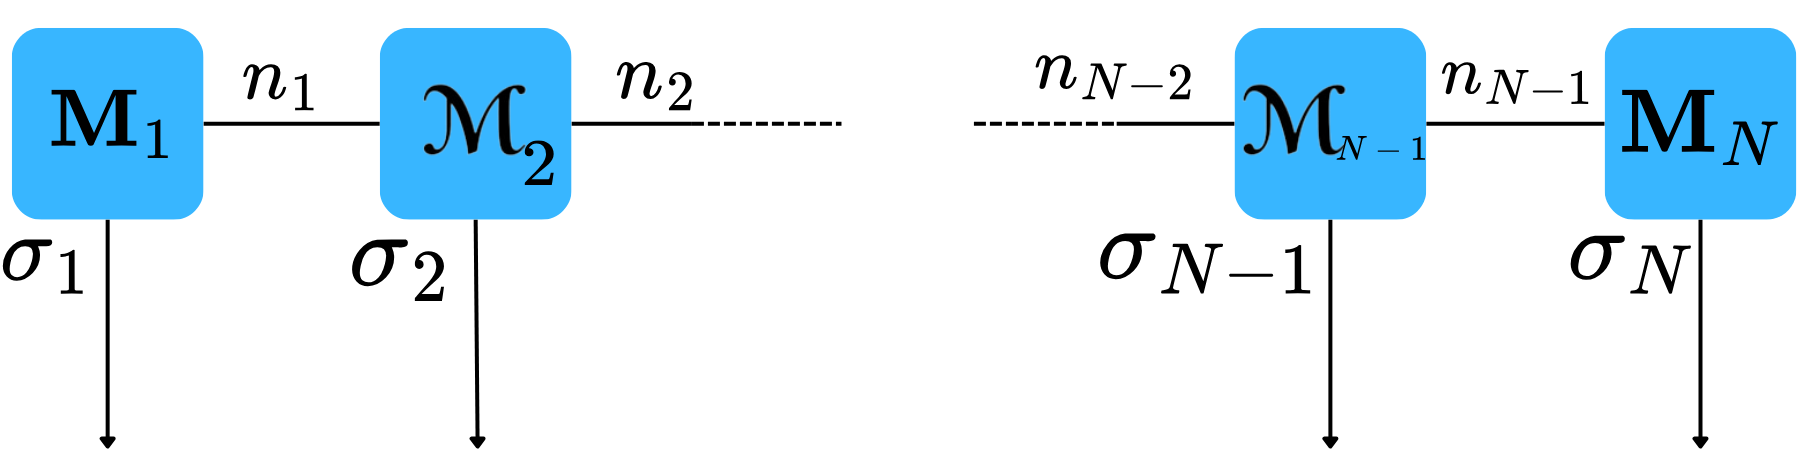
\includegraphics[width=0.9\linewidth]{images/General Tensor Diagrams/MPS_diagram.png}
        \caption{Tensor Diagram of MPS}
        \label{fig:MPS_diagram}
    \end{figure}
\end{frame}


\begin{frame}{Tensor Orthogonality}
    \scriptsize
    \centering
    \setlength\fboxsep{5pt} % Padding between frame and image
    \setlength\fboxrule{0.5pt} % Thickness of frame

    \begin{minipage}{0.32\textwidth}
        \centering
        \begin{figure}
            \centering
            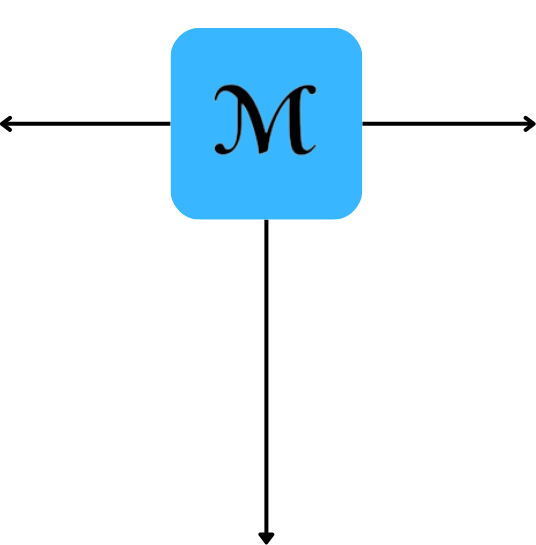
\includegraphics[height = 0.6\linewidth]{images/General Tensor Diagrams/M_tensor_2.png}
            \caption*{Non-Orthogonal}
            \label{fig:M_tensor}
        \end{figure}
    \end{minipage}
        \hfill
    \begin{minipage}{0.32\textwidth}
        \centering
        \begin{figure}
            \centering
            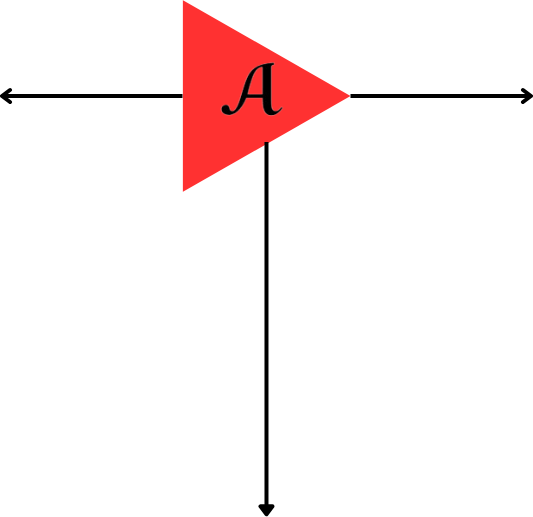
\includegraphics[height = 0.6\linewidth]{images/General Tensor Diagrams/A_tensor.png}
            \caption*{Left-Orthogonal}
            \label{fig:enter-label}
        \end{figure}
        % \caption{Left-Orthogonal Tensor}
    \end{minipage}
        \hfill
    \begin{minipage}{0.32\textwidth}
        \centering
        \begin{figure}
            \centering
            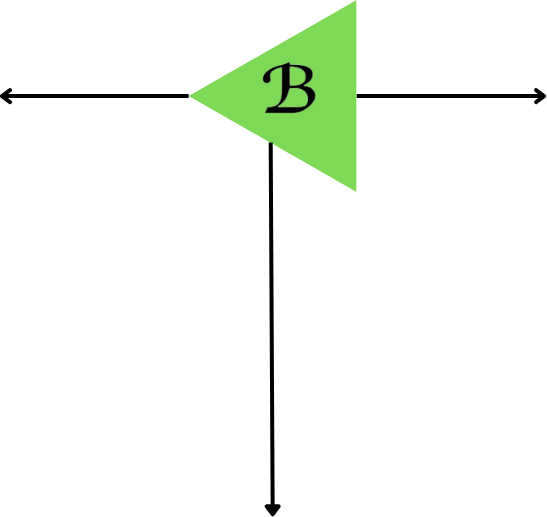
\includegraphics[height = 0.6\linewidth]{images/General Tensor Diagrams/B_tensor.png}
            \caption*{Right-Orthogonal}
            \label{fig:enter-label}
        \end{figure}
        % \caption{Right Orthogonal Tensor}
    \end{minipage}
    \\
    \pause
    \begin{minipage}{0.45\textwidth}
        \centering
        \fbox{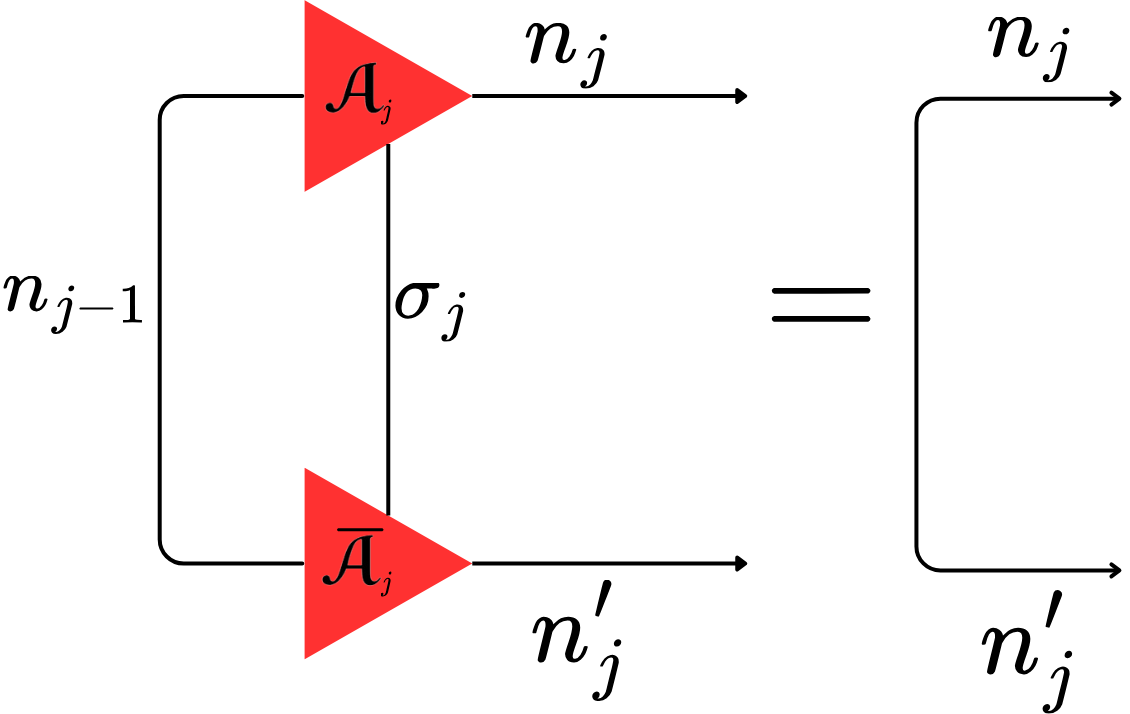
\includegraphics[width=\linewidth]{images/MPS Orthogonality/L_ortho.png}}\\
        \vspace{0.3em}
        Left-Orthogonality: $\sum_{\sigma_j}(\romanL{A}_j^{\sigma_j})^{\dag}\romanL{A}_j^{\sigma_j} = I$
    \end{minipage}
    \hfill
    \begin{minipage}{0.45\textwidth}
        \centering
        \fbox{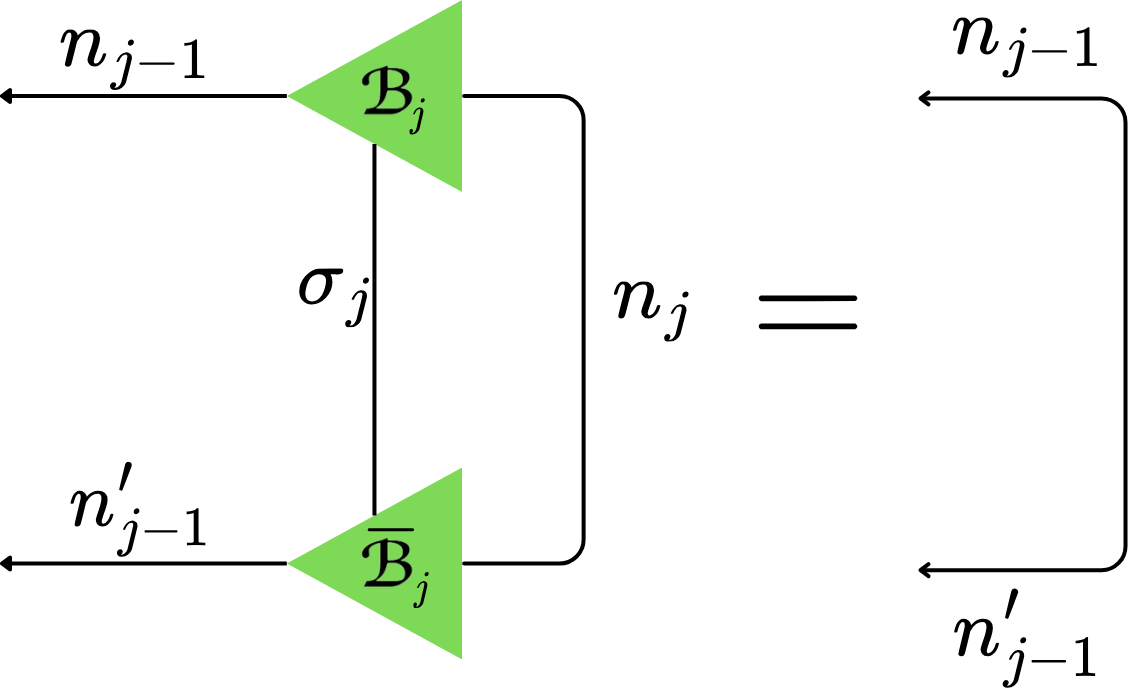
\includegraphics[width=\linewidth]{images/MPS Orthogonality/Right_ortho.png}}\\
        \vspace{0.3em}
        Right-Orthogonality: $\sum_{\sigma_j}\romanL{B}_j^{\sigma_j}(\romanL{B}_j^{\sigma_j})^{\dag} = I$
    \end{minipage}
    \blfootnote{\citetitle{PAECKEL2019167998}}
\end{frame}

\begin{frame}{Matrix Product State Canonical Forms}
    \small
    % Matrix product states can be in certain forms: left-orthogonal canonical form, right-orthogonal canonical form, and mixed canonical form. 
    \begin{itemize}[<+->]
        \item Left-Orthogonal canonical form: 
            \begin{figure}
                \centering
                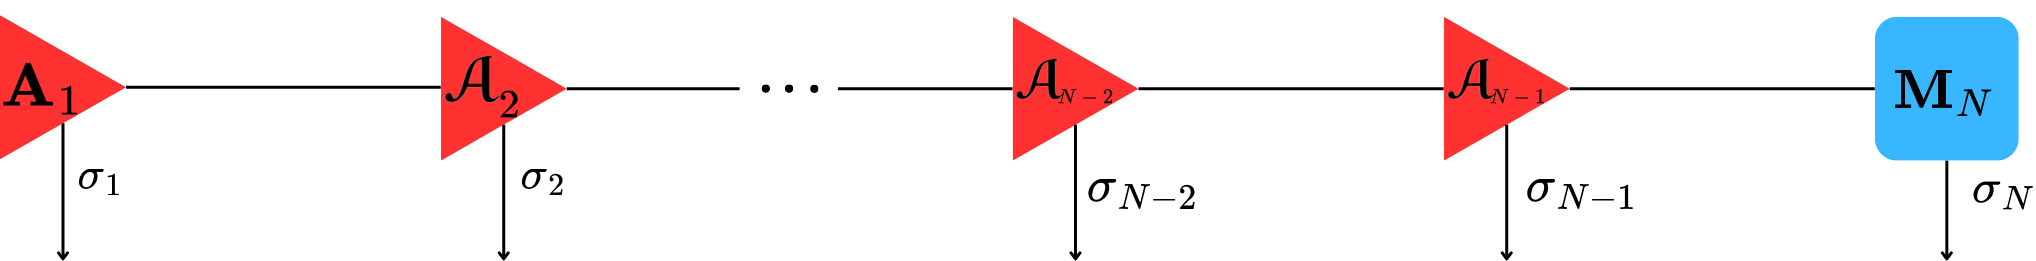
\includegraphics[width=0.8\linewidth]{images/MPS Orthogonality/L_canonical_short.png}
                \caption*{$|\psi\rangle = \sum_{\boldsymbol{\sigma}}\romanL{a}_1^{\sigma_1}\romanL{A}_2^{\sigma_2}...\romanL{A}_{N - 1}^{\sigma_{N - 1}}\romanL{m}_N^{\sigma_N}|\boldsymbol{\sigma}\rangle, \quad$}
                \label{fig:enter-label}
            \end{figure}
        \vspace{-15pt}
        \item Right-Orthogonal canonical form:
        \begin{figure}
            \centering
            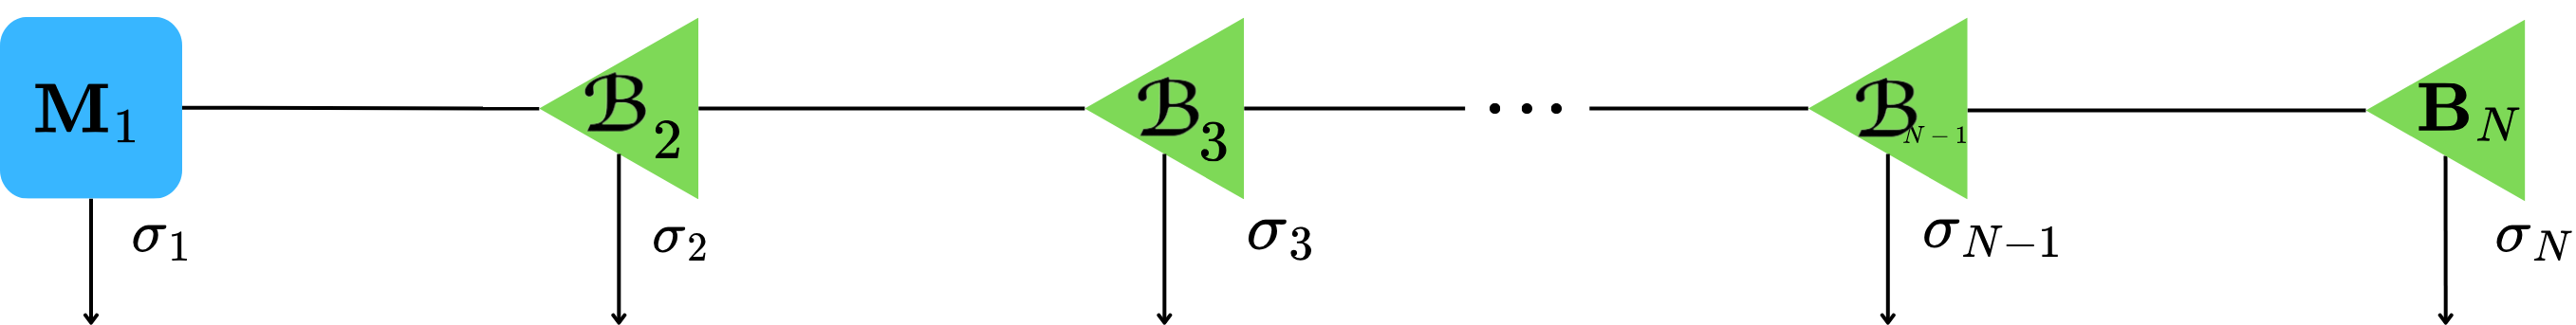
\includegraphics[width=0.8\linewidth]{images/MPS Orthogonality/Right_canonical.png}
            \caption*{$|\psi\rangle = \sum_{\boldsymbol{\sigma}}\romanL{m}_1^{\sigma_1}\romanL{B}_2^{\sigma_2}...\romanL{B}_{N - 1}^{\sigma_{N - 1}}\romanL{b}_N^{\sigma_N}|\boldsymbol{\sigma}\rangle,\quad$}
            \label{fig:enter-label}
        \end{figure}
        \vspace{-15pt}
        \item Mixed-Orthogonal canonical form:
        
        \begin{figure}
            \centering
            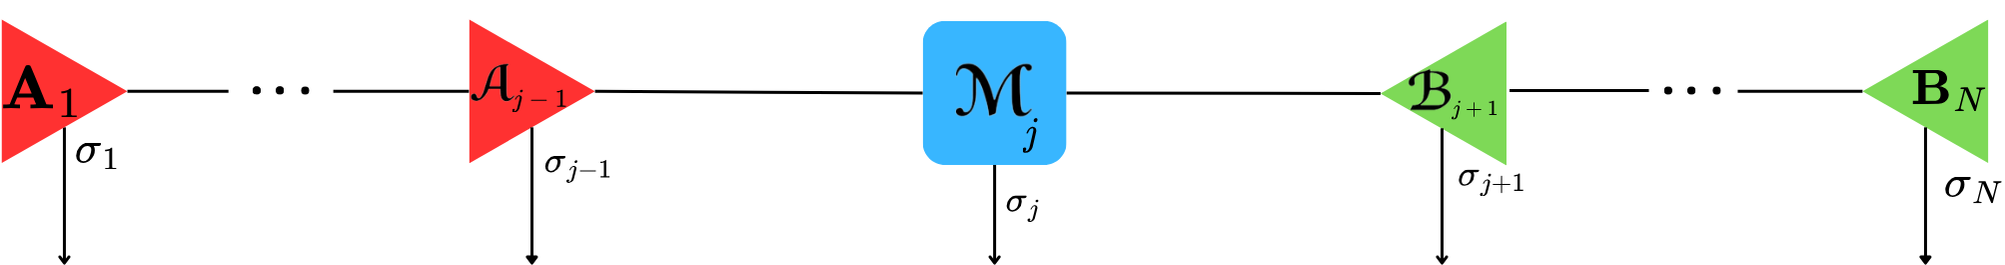
\includegraphics[width=0.8\linewidth]{images/MPS Orthogonality/M_canonical_short.png}
            \caption*{$|\psi\rangle = \sum_{\boldsymbol{\sigma}}\romanL{a}_1^{\sigma_1}...\romanL{A}_{\ell - 1}^{\sigma_{\ell - 1}}\romanL{M}_\ell^{\sigma_\ell}\romanL{B}_{\ell + 1}^{\sigma_{\ell + 1}}...\romanL{b}_N^{\sigma_N}|\boldsymbol{\sigma}\rangle.$}
            \label{fig:mixed_canonical}
        \end{figure}
    \end{itemize}
    \footnote{\citetitle{SCHOLLWOCK201196}}
\end{frame}



\begin{frame}{Usefulness of Canonical Forms}
    \small
    Let's take the inner product of a quantum state with itself, $\langle\psi|\psi\rangle$, as a tensor diagram we have: \begin{figure}
        \centering
        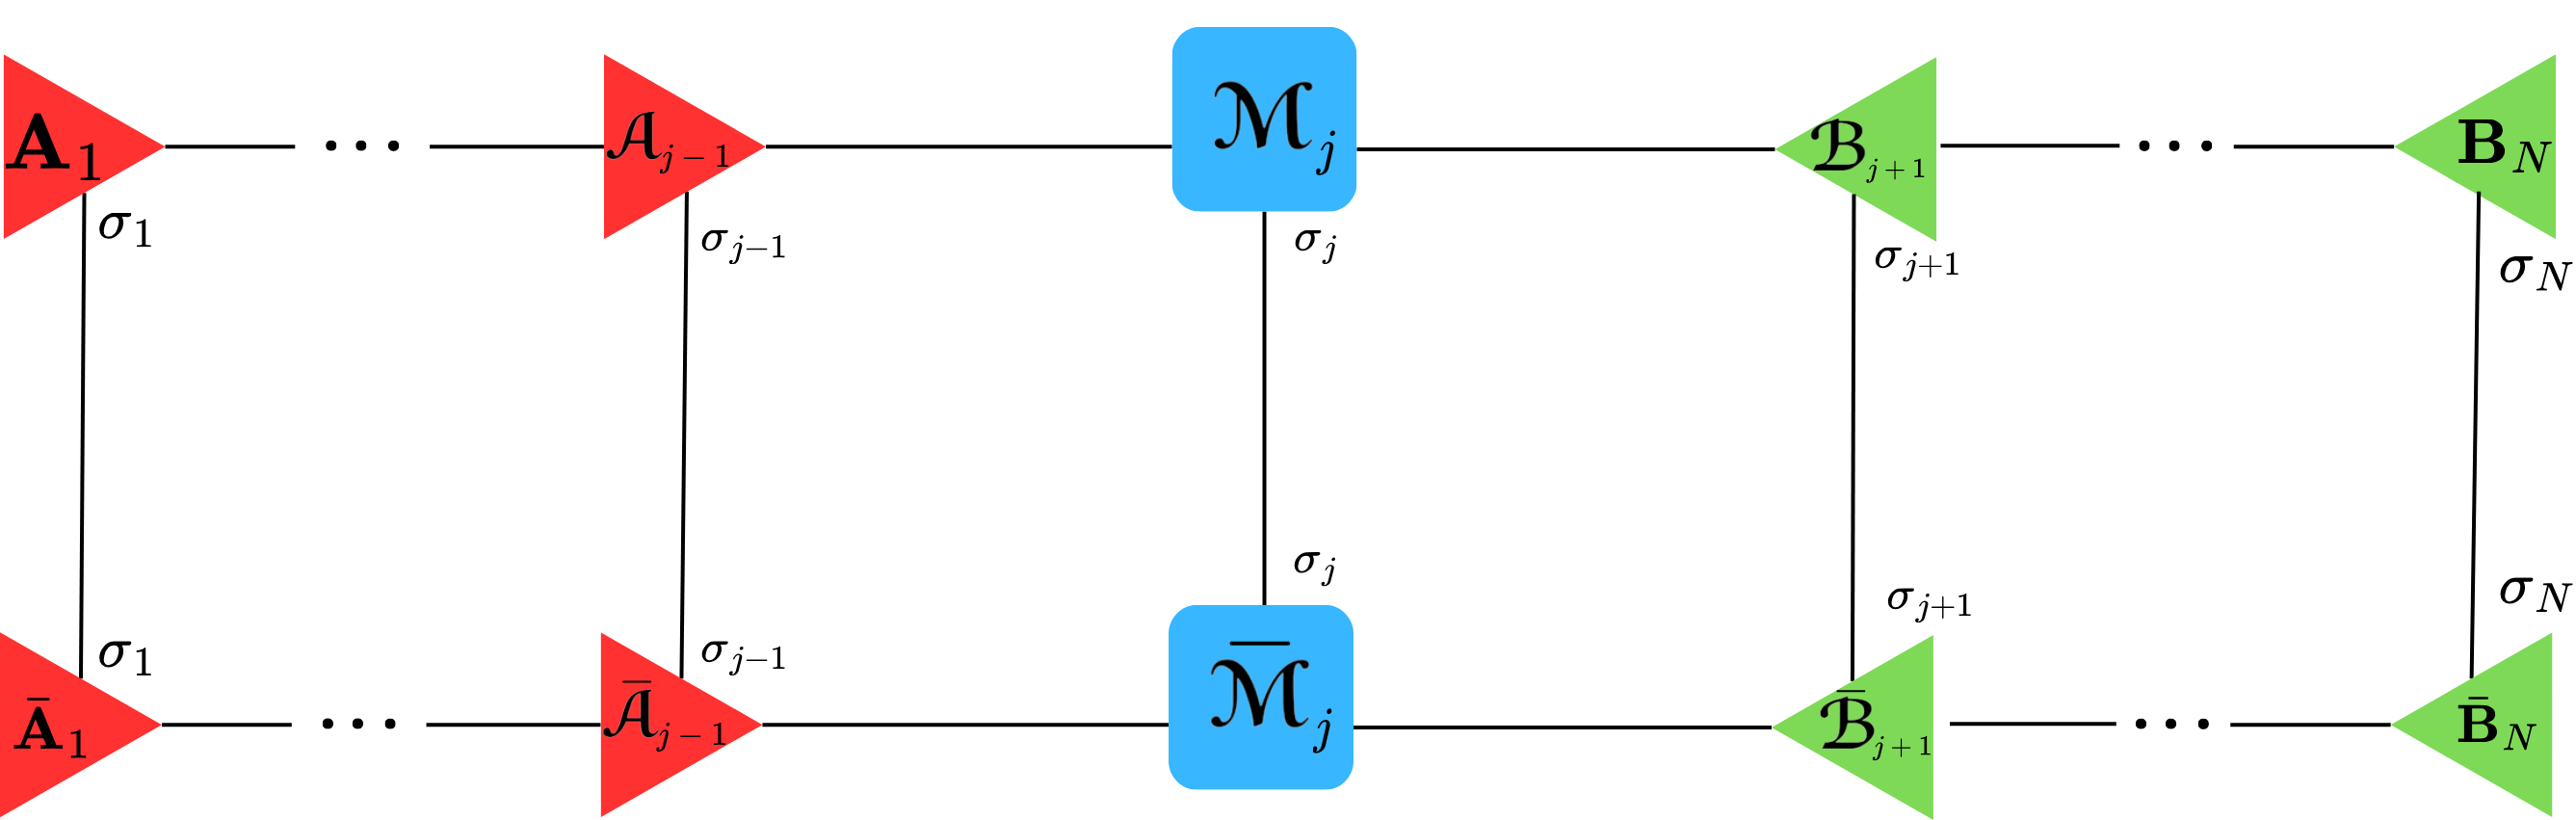
\includegraphics[width=0.8\linewidth]{images/MPS Orthogonality/MPS_IP.png}
        \small \caption{\small Inner Product of $\langle\psi|\psi\rangle$}
        \label{fig:enter-label}
    \end{figure}
    \pause
        \begin{figure}
            \centering
            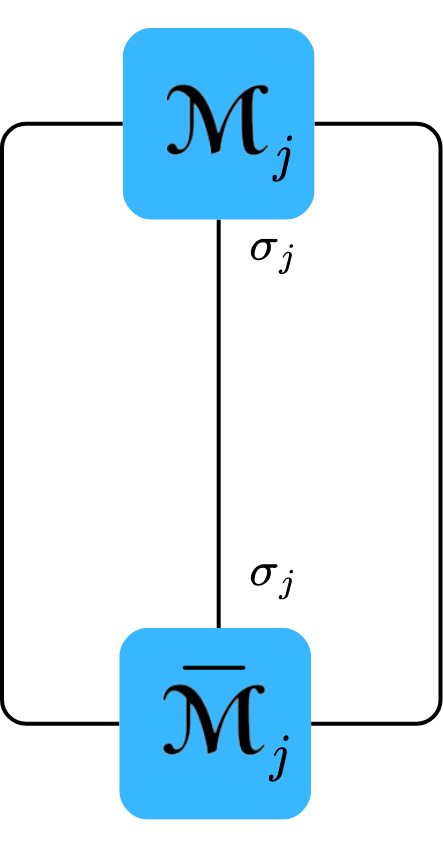
\includegraphics[scale = 0.116]{images/MPS Orthogonality/MPS_IP_2.png}
            \small\caption{\small $\langle \psi|\psi\rangle = ||M_j||^2_F$}
            \label{fig:enter-label}
        \end{figure}
    \blfootnote{\citetitle{PAECKEL2019167998}}
\end{frame}

\begin{frame}{Calculating the MPS}
    \includegraphics<1>[width = \linewidth]{images/MPS Creation/MPS_beginning.png}
    \includegraphics<2>[width = \linewidth]{images/MPS Creation/MPS_Step2_QR.png}
    \includegraphics<3>[width = \linewidth]{images/MPS Creation/MPS_FinalStep_QR.png}
    \only<1>{\centering \small Initial Tensor}
    \only<2>{\centering \small Performing QR decomposition}
    \only<3>{\centering \small Final State as MPS}
\end{frame}


\begin{frame}{Matrix Product State (MPS) Storage}
    For $N$ qubits:\\ 
    \vspace{1cm}
        \begin{tabular}{c|c}
             \textbf{Vector Storage} & \textbf{MPS Storage} \\
             \hline
             Storage exponential with $N$ & Storage linear in $N$\\
              & May require large bond dimension\\[0.5cm]
              \pause
              $2^N$ complex numbers stored & $>2^{N + 1}$ complex numbers stored\\
              \hline
            
        \end{tabular}
    \pause
    
    \vspace{1cm}
            Key idea: truncate matrix dimensions via SVD
            \begin{itemize}
                \item High entanglement $\Rightarrow$ Larger bond dimension
                \item Low entanglement $\Rightarrow$ Smaller bond dimension
            \end{itemize}
    \blfootnote{\citetitle{SCHOLLWOCK201196}}
\end{frame}

\begin{frame}{MPS Truncation}
    \small
    A separable state (e.g., $|0\rangle \otimes |0\rangle \otimes ...\otimes |0\rangle$ can be represented with much smaller storage:

    \vspace{0.5em}
    \begin{figure}
        \centering
        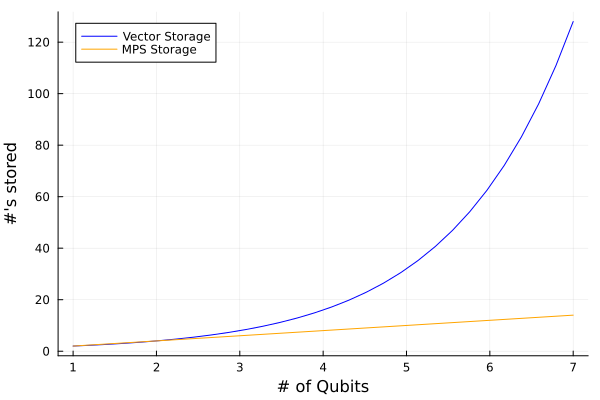
\includegraphics[width=0.8\linewidth]{images/Misc/total_scale.png}
        \caption{Separable State Storage}
        \label{fig:Total_Scale}
    \end{figure}

\end{frame}


\begin{frame}{Truncating MPS via SVD}
  \begin{itemize}
    \item To control bond dimensions, we truncate tensors by performing an SVD of one of the core tensors.
  \end{itemize}



  \vspace{0.5em}
  \begin{itemize}
    \item Truncate by keeping only largest $\chi$ singular values: $\lambda_1 \geq \dots \geq \lambda_\chi$
    \item Truncation error: $\epsilon_{\text{trunc}} = \sqrt{\sum_{s>\chi} \lambda_s^2}$
  \end{itemize}
  \blfootnote{\citetitle{SCHOLLWOCK201196}}
\end{frame}

\begin{frame}{SVD Truncation}
    \includegraphics<1>[width = 0.95\linewidth]{images/Truncate/Truncate1.png}
    \includegraphics<2>[width = 0.95\linewidth]{images/Truncate/Truncate2_USV_2.png}
    \includegraphics<3>[width = 0.95\linewidth]{images/Truncate/Truncate3_USV_2.png}
    \includegraphics<4>[width = 0.95\linewidth]{images/Truncate/Truncate4.png}
    \includegraphics<5>[width = 0.95\linewidth]{images/Truncate/Truncate5_USV_2.png}
    \includegraphics<6>[width = 0.95\linewidth]{images/Truncate/Truncate6_USV_2.png}
    \includegraphics<7>[width = 0.95\linewidth]{images/Truncate/Truncate7.png}
    \only<1>{\centering \small Initial state with bond dimensions $n_1$, $n_2$}
    \only<2>{\centering \small SVD performed on $\romanL{M}_1$}
    \only<3>{\centering \small Truncation of Singular value matrix, $\romanL{S}_1$}
    \only<4>{\centering \small Tensor contraction of $\romanL{S}_1^*, \romanL{V}_1, \euler{B}_2$}
    \only<5>{\centering \small SVD of $\euler{M}_2$}
    \only<6>{\centering \small Truncation of singular value matrix, $\romanL{S}_2$}
    \only<7>{\centering \small Tensor contraction of $\romanL{S}_2^*, \romanL{V}_2, \romanL{B}_3$}
\end{frame}

\begin{frame}{Matrix Product Operator (MPO)}
    \small
    To evolve an MPS under Schrödinger's equation,
    \[
        |\dot{\psi}\rangle = -iH|\psi\rangle,
    \]
    we express the Hamiltonian $H$ as a Matrix Product Operator (MPO)—a tensor train of order-3 and order-4 tensors. As a tensor diagram: 

    \begin{figure}
        \centering
        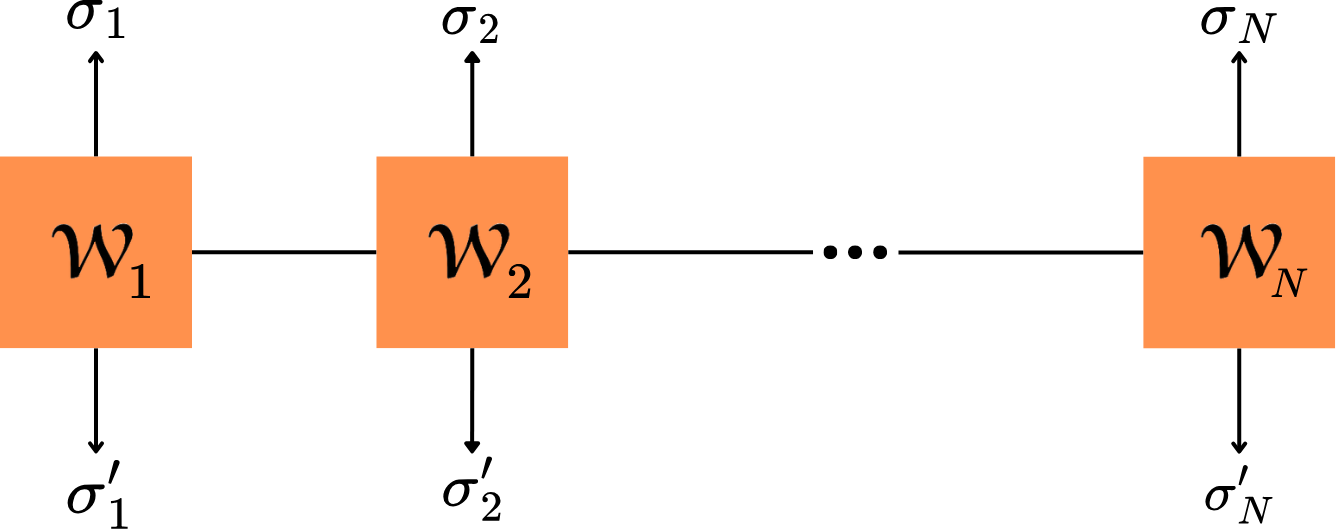
\includegraphics[width=0.65\linewidth]{images/General Tensor Diagrams/MPO_2.png}
        \caption{Diagram notation of an MPO}
    \end{figure}
    \blfootnote{\citetitle{SCHOLLWOCK201196}}
\end{frame}


\begin{frame}{MPS/MPO Operations and Bond Dimension Growth}
  \small
  Key operations that increase bond dimension:
  \begin{itemize}
    \item \textbf{MPS Addition:} Adding two MPS increases bond dimension:
    \[
      \ell_i = m_i + n_i
    \]
    \item \textbf{MPO Application:} Applying an MPO to an MPS multiplies bond dimensions:
    \[
      \ell_i = w_i \cdot n_i
    \]
  \end{itemize}

  \vspace{0.5em}
  Both operations lead to higher computational cost due to bond dimension growth.
  \blfootnote{\citetitle{SCHOLLWOCK201196}}
\end{frame}


\AtBeginSection[]
{
  \begin{frame}
    \frametitle{Table of Contents}
    \tableofcontents[currentsection]
  \end{frame}
}
\section{Matrix Product State Evolution}

\begin{frame}{MPS Time Evolution Methods}
\small
\begin{tabular}{|p{2cm}|p{4.0cm}|p{4.0cm}|}
\hline
\textbf{Method} & \textbf{Pros} & \textbf{Cons} \\
\hline
TEBD & Easy to implement for local Hamiltonians & Not effective for long-range Hamiltonians\\
\hline
$W^{I, II}$ & Allows long-range Hamiltonians, typically 
smaller bond dimension than TEBD & Evolution not unitary \\
\hline

Krylov Method & High accuracy, flexible for different Hamiltonians & Quickly increases bond dimension\\
\hline
TDVP & Preservation of norm, Fixed Bond Dimension & Fixed Bond Dimension \\
\hline
TDVP2 & Allows bond dimension growth, handles entanglement better & More computationally expensive, doesn't necessarily preserve norm\\
\hline

\end{tabular}
\blfootnote{\citetitle{PAECKEL2019167998}}
\end{frame}

\begin{frame}{TDVP Evolution Picture}
    \small
    The Time-Dependent Variational Principle (TDVP) evolves Schrödinger's equation within the manifold of MPS with fixed bond dimension by projecting onto the tangent space:
    \begin{figure}
        \centering
        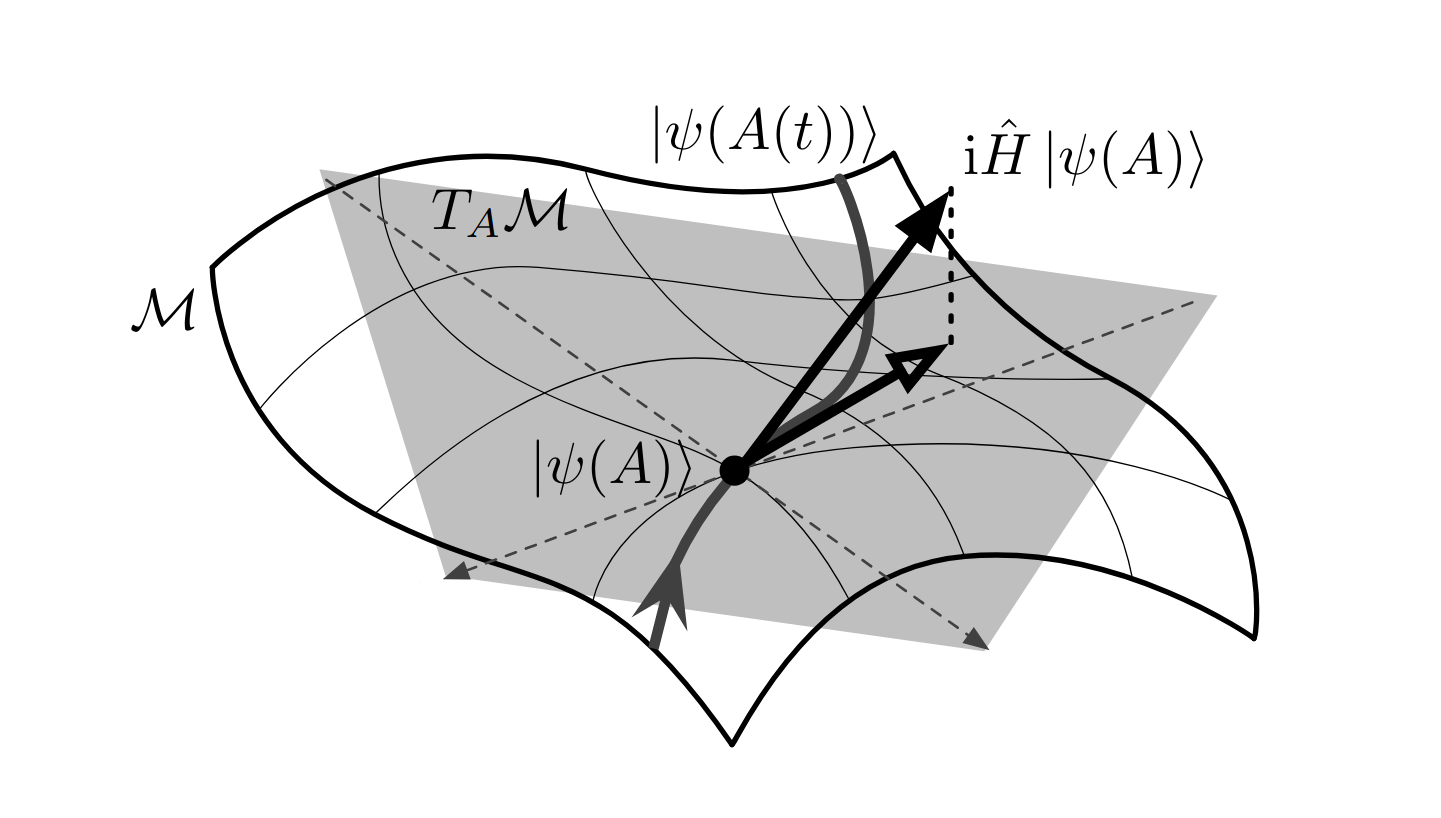
\includegraphics[width=0.8\linewidth]{images/Misc/Manifold.png}
        \caption{Projection}
        \label{fig:Projection}
    \end{figure}
    \blfootnote{\citetitle{PhysRevLett.107.070601}}
\end{frame}

\begin{frame}{TDVP Evolution}
    \begin{equation}
        |\dot{\psi}\rangle = -iP_{T, |\psi\rangle}H|\psi\rangle
    \end{equation}
    \pause
    The projector $P_{T, |\psi\rangle}$ decomposes into a sum of local projectors:
    \begin{align*}
        &P_{T, |\psi\rangle} = \sum_{i = 1}^N P_i^+ - \sum_{i= 1}^{N - 1} P_i^-\\
        &P_{T, |\psi\rangle} = P^{+}_1 - P^{-}_1 + P_2^{+}- P_2^{-} + ... - P_{N - 1}^{-} + P_{N}^{+}
    \end{align*}
    \pause
    \vspace{0.5em}
    The evolution is performed using a Lie-Trotter splitting scheme, solving one-site and zero-site ODEs:
    
    \begin{center}
    \renewcommand{\arraystretch}{1.6}
    \begin{tabular}{|c|c|c|}
        \hline
        \textbf{Projector Step} & \textbf{Tensor ODE} & \textbf{Vectorized Form} \\
        \hline
        $|\dot{\psi}\rangle = -iP_i^+H|\psi\rangle$ & $\dot{\euler{M}}_i = -i\euler{H}_{\textrm{eff}}^i \euler{M}_i$ & $\dot{\boldsymbol{m}} = -i\romanL{H}_{\textrm{eff}}^i \boldsymbol{m}$ \\
        \hline
        $|\dot{\psi}\rangle = iP_iH^-|\psi\rangle$ & $\dot{\romanL{C}}_i = i\euler{K}_{\textrm{eff}}^i \romanL{C}_i$ & $\dot{\boldsymbol{c}} = i\romanL{K}_{\textrm{eff}}^i \boldsymbol{c}$ \\
        \hline
    \end{tabular}
    \end{center}
    \blfootnote{\citetitle{PhysRevLett.107.070601}}
\end{frame}

\begin{frame}{Effective Hamiltonian}
    \includegraphics<1>[width = 0.9\linewidth]{images/Effective_Hamiltonians/1Site_Eff.png}
    \includegraphics<2>[width = 0.9\linewidth]{images/Effective_Hamiltonians/0Site_Eff.png}
    \only<1>{\centering \small Tensor Diagram of $\euler{H}_{\textrm{eff}}^2$.}
    \only<2>{\centering \small Tensor Diagram of $\euler{K}_{\textrm{eff}}^2$.}
\end{frame}


\begin{frame}{TDVP Evolution Tensor Diagram}
    \includegraphics<1>[width = 0.95\linewidth]{images/TDVP Evolution Tensor/TDVP_Tensor_1.png}
    \includegraphics<2>[width = 0.95\linewidth]{images/TDVP Evolution Tensor/TDVP_Tensor_2.png}
    \includegraphics<3>[width = 0.95\linewidth]{images/TDVP Evolution Tensor/TDVP_Tensor_3.png}
    \includegraphics<4>[width = 0.95\linewidth]{images/TDVP Evolution Tensor/TDVP_Tensor_4.png}
    \includegraphics<5>[width = 0.95\linewidth]{images/TDVP Evolution Tensor/TDVP_Tensor_5.png}
    \includegraphics<6>[width = 0.95\linewidth]{images/TDVP Evolution Tensor/TDVP_Tensor_6.png}
    \includegraphics<7>[width = 0.95\linewidth]{images/TDVP Evolution Tensor/TDVP_Tensor_7.png}
    \includegraphics<8>[width = 0.95\linewidth]{images/TDVP Evolution Tensor/TDVP_Tensor_8.png}
    \includegraphics<9>[width = 0.95\linewidth]{images/TDVP Evolution Tensor/TDVP_Tensor_9.png}
    \includegraphics<10>[width = 0.95\linewidth]{images/TDVP Evolution Tensor/TDVP_Tensor_10.png}
\end{frame}

\begin{frame}{TDVP Evolution Example: CNOT gate}
    The CNOT quantum gate (short for Controlled NOT), swaps the states $|10\rangle$ and $|11\rangle$, and leaves the states $|00\rangle$ and $|01\rangle$ unchanged.
    \begin{equation*}
        CNOT|10\rangle = |11\rangle, \quad CNOT|11\rangle = |10\rangle.
    \end{equation*} 
    \pause
    As a matrix: $$CNOT = \begin{bmatrix}
        1 & 0 & 0 & 0\\
        0 & 1 & 0 & 0\\
        0 & 0 & 0 & 1\\
        0 & 0 & 1 & 0
    \end{bmatrix}$$
    The CNOT gate control pulses were computed using the quantum control package \textit{quandary}. 

\end{frame}
\begin{frame}{TDVP Evolution Example: CNOT gate}
    \includegraphics<1>[width = 0.9\linewidth]{images/TDVP_Evolution/TDVP_EvolutionBD4_2.png}
    \includegraphics<2>[width = 0.9\linewidth]{images/TDVP_Evolution/TDVP_EvolutionBD3_2.png}
    \includegraphics<3>[width = 0.9\linewidth]{images/TDVP_Evolution/TDVP_EvolutionBD2_2.png}
    \includegraphics<4>[width = 0.9\linewidth]{images/TDVP_Evolution/TDVP_EvolutionBD1_2.png}
\end{frame}

\begin{frame}{2 Site TDVP Evolution}
    \small
    \begin{equation}
        |\dot{\psi}\rangle = -iP_{T_2, |\psi\rangle}H|\psi\rangle
    \end{equation}
    \pause
    2 site TDVP Evolution (TDVP2) evolves Schrödinger's equation, but by evolving two sites at one time, then splitting them up via SVD. This allows bond dimension growth.     
    
    The projector $P_{T_2, |\psi\rangle}$ is a sum of projectors on individual sites of the MPS. 
    \begin{align}
        &P_{T_2, |\psi\rangle} = \sum_{i = 1}^{N - 1}P_i^{+} - \sum_{i = 2}^{N - 2}P_i^{-}\nonumber, \\ 
        &P_{T_2, |\psi\rangle} = P^{+}_1 - P^{-}_2 + P_2^{+}-P_3^{-} + ... - P_{N - 2}^{-} + P_{N-1}^{+}.
    \end{align}    
    \pause
    The evolution is performed using a Lie-Trotter splitting scheme, solving two-site and one-site ODEs:
    \begin{center}
    \renewcommand{\arraystretch}{1.6}
    \begin{tabular}{|c|c|c|}
        \hline
        \textbf{Projector Step} & \textbf{Tensor ODE} & \textbf{Vectorized Form} \\
        \hline
        $|\dot{\psi}\rangle = -iP_i^+H|\psi\rangle$ & $\dot{\euler{M}}_{i,i + 1} = -i\euler{H}_{\textrm{eff}}^{i, i + 1} \euler{M}_{i, i + 1}$ & $\dot{\boldsymbol{m}} = -i\romanL{H}_{\textrm{eff}}^{i, i + 1} \boldsymbol{m}$ \\
        \hline
        $|\dot{\psi}\rangle = iP_i^-H|\psi\rangle$ & $\dot{\euler{M}}_i= i\euler{H}_{\textrm{eff}}^i \euler{M}_i$ & $\dot{\boldsymbol{m}} = i\romanL{H}_{\textrm{eff}}^i \boldsymbol{m}$ \\
        \hline
    \end{tabular}
    \end{center}
    \blfootnote{\citetitle{PhysRevLett.107.070601}
    }
\end{frame}

\begin{frame}{2 site Effective Hamiltonian}

    \begin{figure}
        \centering
        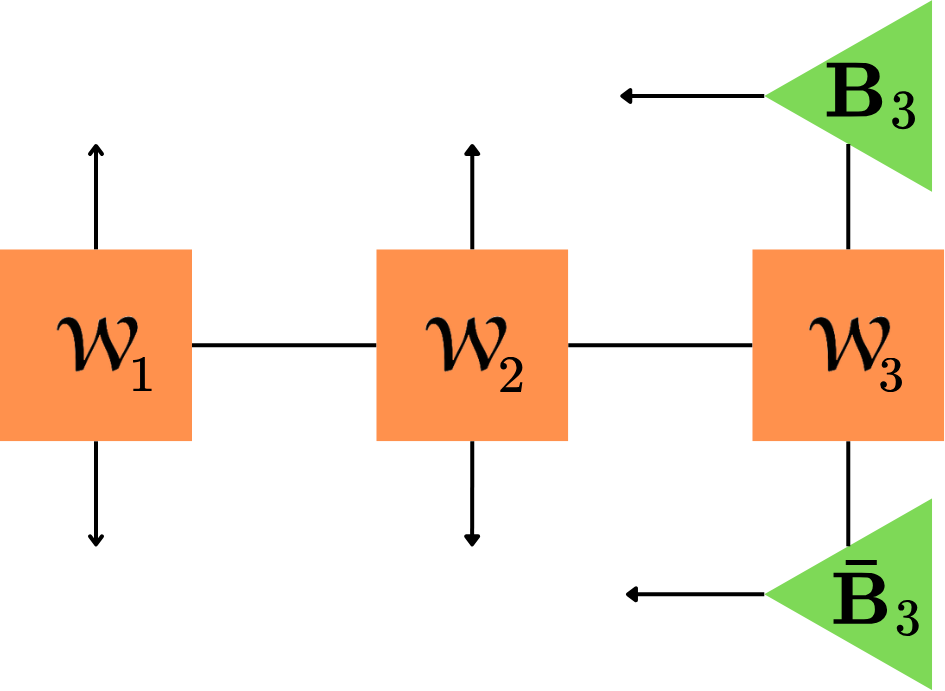
\includegraphics[width=0.7\linewidth]{images/Effective_Hamiltonians/2Site_Eff.png}
        \caption{Tensor Diagram of $\euler{H}_{\textrm{eff}}^{1,2}$.}
        \label{fig:Keff}
    \end{figure}
\end{frame}

\begin{frame}{TDVP2 Evolution Tensor Diagram}
    \includegraphics<1>[width = 0.95\linewidth]{images/TDVP2 Tensor Diagram/TDVP2_Tensor_1.png}
    \includegraphics<2>[width = 0.95\linewidth]{images/TDVP2 Tensor Diagram/TDVP2_Tensor_2.png}
    \includegraphics<3>[width = 0.95\linewidth]{images/TDVP2 Tensor Diagram/TDVP2_Tensor_3.png}
    \includegraphics<4>[width = 0.95\linewidth]{images/TDVP2 Tensor Diagram/TDVP2_Tensor_4.png}
    \includegraphics<5>[width = 0.95\linewidth]{images/TDVP2 Tensor Diagram/TDVP2_Tensor_5.png}
    \includegraphics<6>[width = 0.95\linewidth]{images/TDVP2 Tensor Diagram/TDVP2_Tensor_6.png}
    \includegraphics<7>[width = 0.95\linewidth]{images/TDVP2 Tensor Diagram/TDVP2_Tensor_7.png}
    \includegraphics<8>[width = 0.95\linewidth]{images/TDVP2 Tensor Diagram/TDVP2_Tensor_8.png}
\end{frame}

\begin{frame}{TDVP2 Evolution}
    \fontsize{10pt}{7.2pt}\selectfont
    \begin{figure}
        \centering
        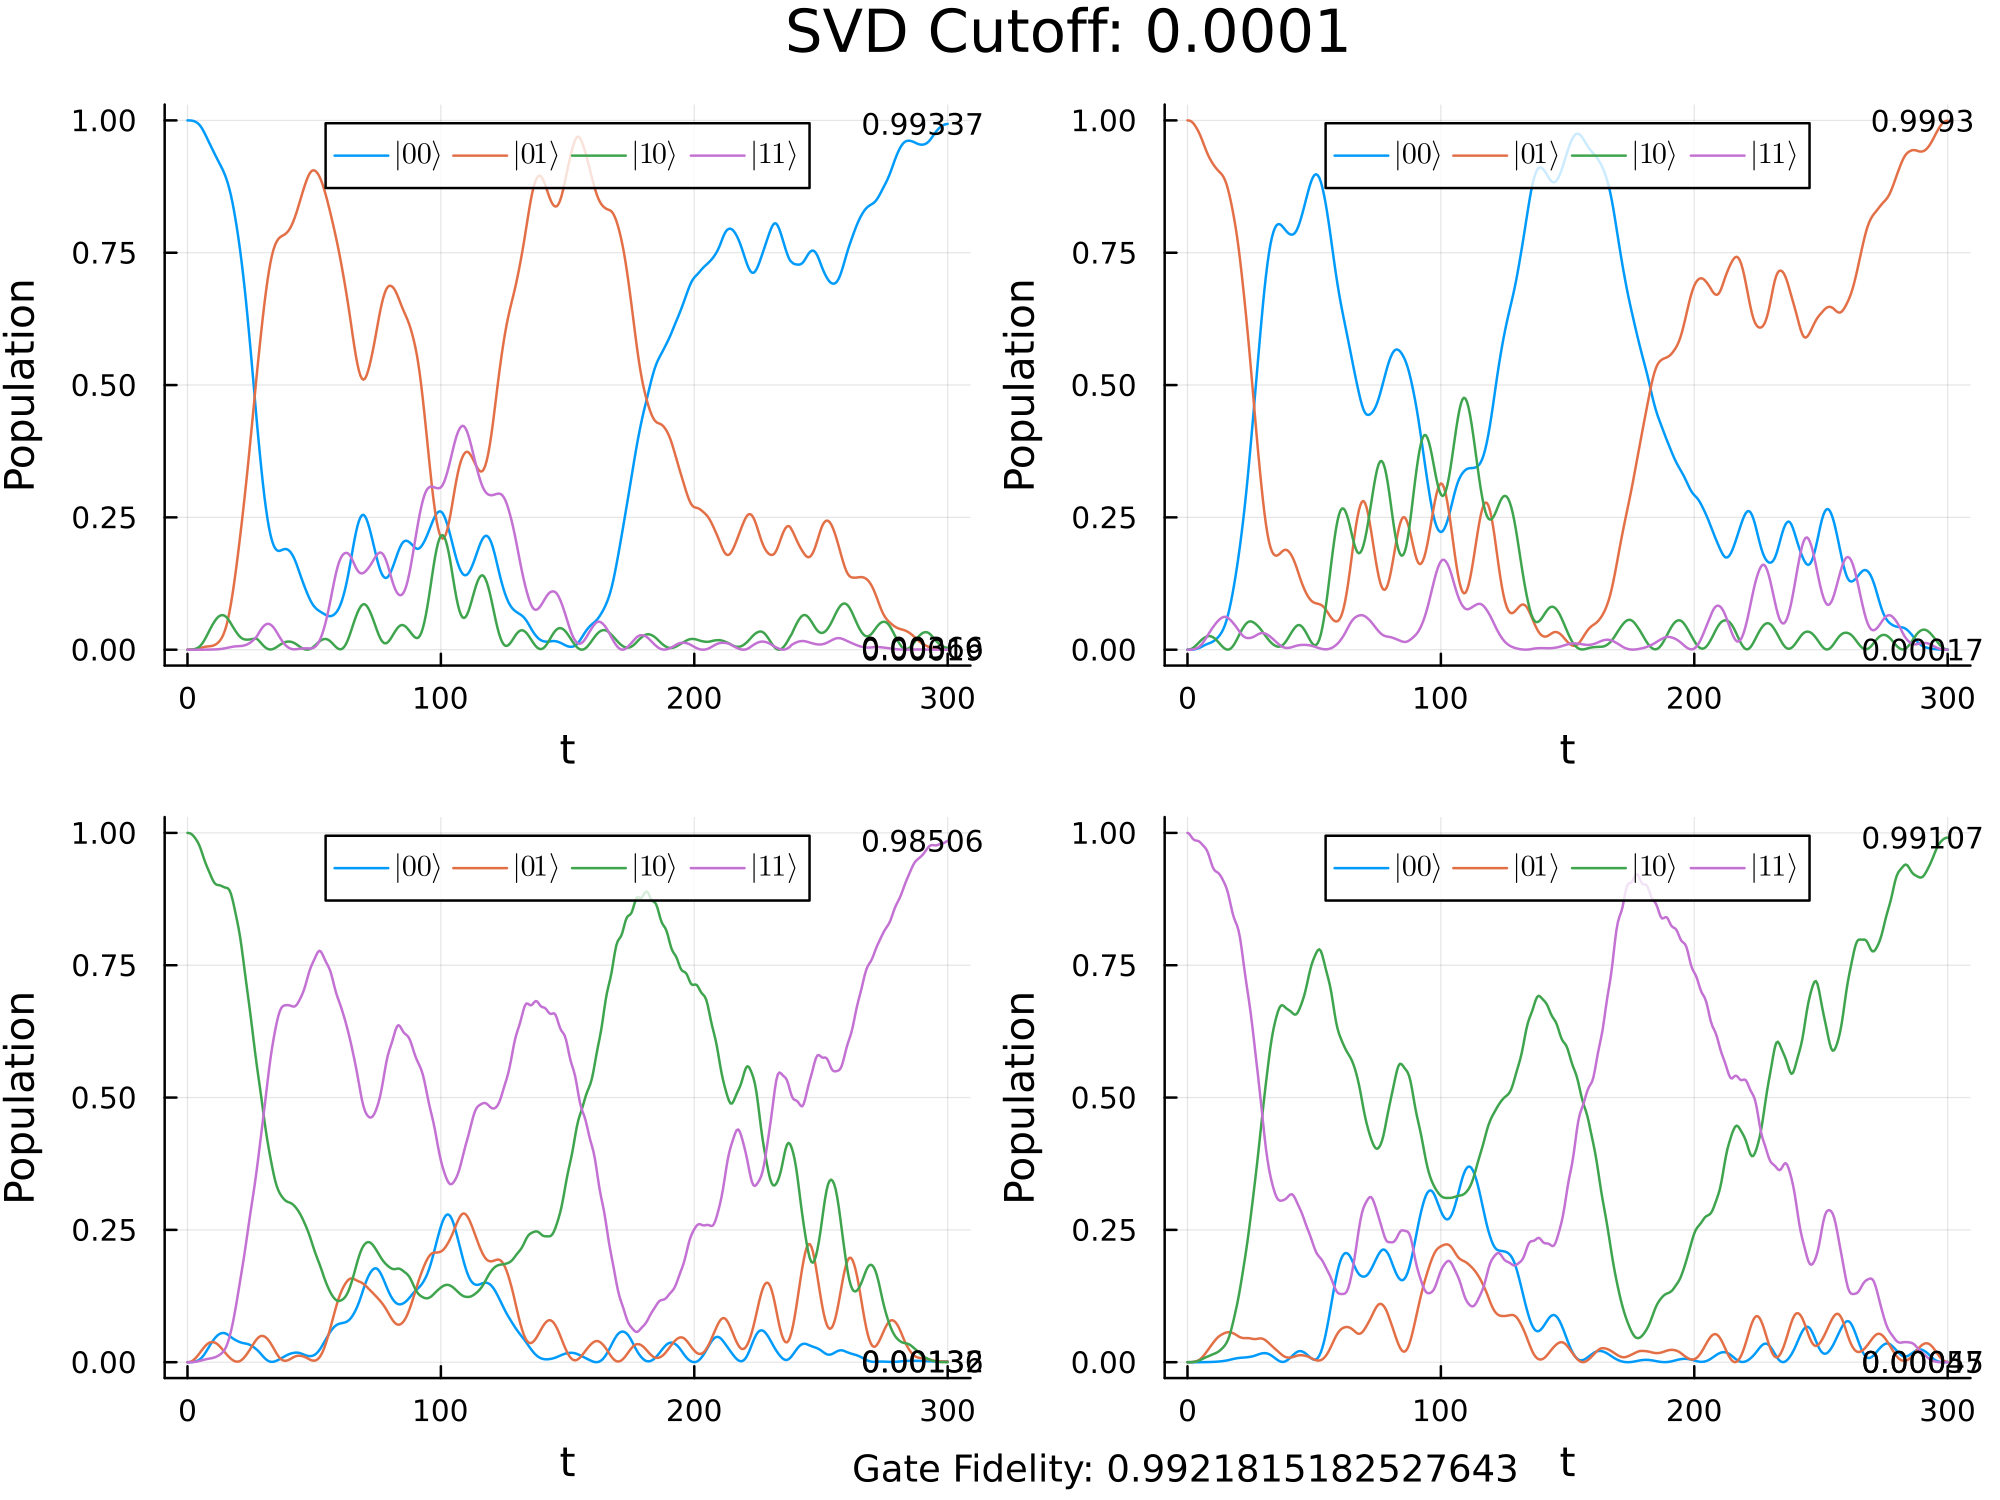
\includegraphics[width=0.9\linewidth]{images/TDVP2 Tensor Diagram/TDVP2_Evolution.png}
        \caption{TDVP2 Evolution with SVD cutoff of 1E-4}
        \label{fig:TDVP2_Evolution}
    \end{figure}

\end{frame} 

\begin{frame}{TDVP2 Evolution}
    \fontsize{10pt}{7.2pt}\selectfont 
    \begin{figure}
        \centering
        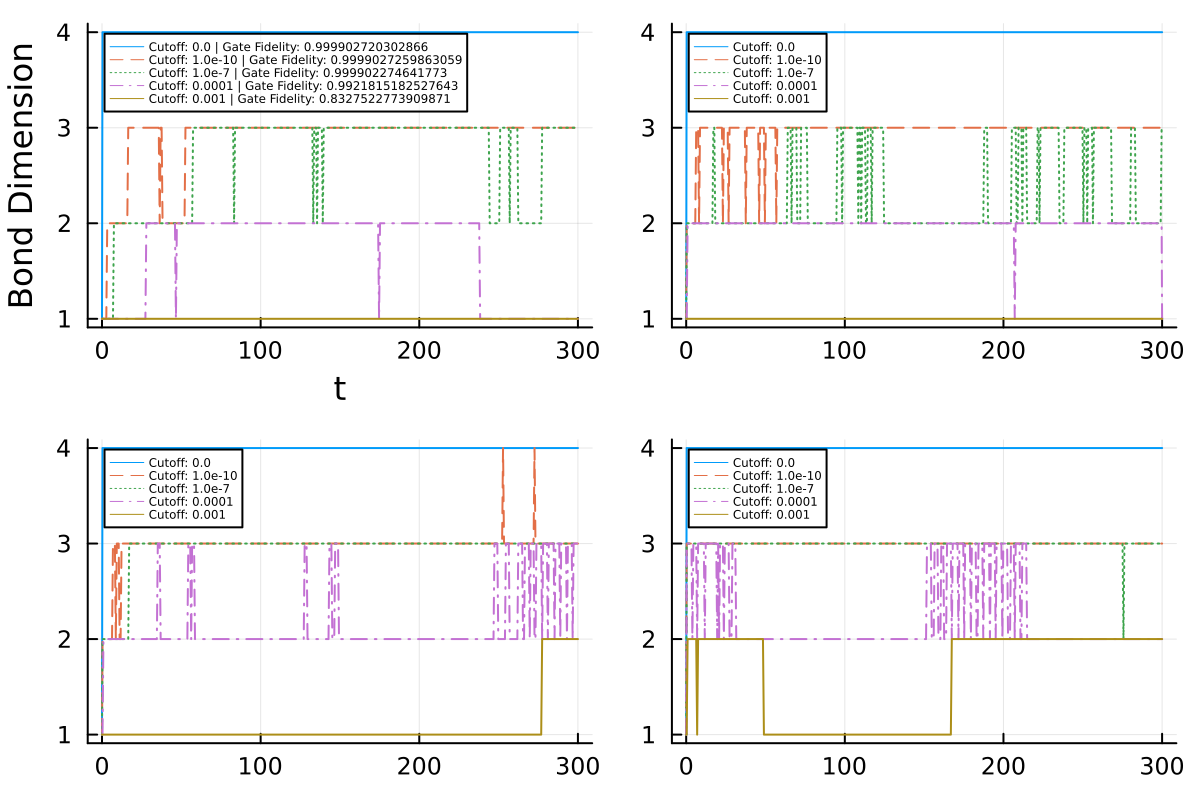
\includegraphics[width=0.95\linewidth]{images/TDVP2 Tensor Diagram/bd_plot.png}
        \caption{Change in bond dimension for different SVD cutoff values for TDVP2.}
        \label{fig:TDVP2_BondDimension}
    \end{figure}
\end{frame}

\begin{frame}{TDVP Error}
    Three Sources of Error: 
    \begin{itemize}
        \item Projection Error \begin{equation*}
            ||H|\psi\rangle - P_{T, |\psi\rangle}H|\psi\rangle||_2
        \end{equation*}
        \item Splitting Error from ODE splitting Method
        \item Truncation Error (for TDVP2) 
    \end{itemize}
    \blfootnote{\citetitle{PhysRevLett.107.070601}}
\end{frame}

\AtBeginSection[]
{
  \begin{frame}
    \frametitle{Table of Contents}
    \tableofcontents[currentsection]
  \end{frame}
}
\section{Future Direction}
\begin{frame}{Develop Method for continuous time Hamiltonian}
    We solve the equation \begin{equation*}
        |\dot{\psi}\rangle = -iH(t)|\psi\rangle,
    \end{equation*}
    with 
    \begin{equation*}
        H(t) = H_s + H_c(t).
    \end{equation*}
    \pause
    The pulses implemented for the CNOT gate were done as piecewise constant pulses.
    \begin{figure}
        \centering
        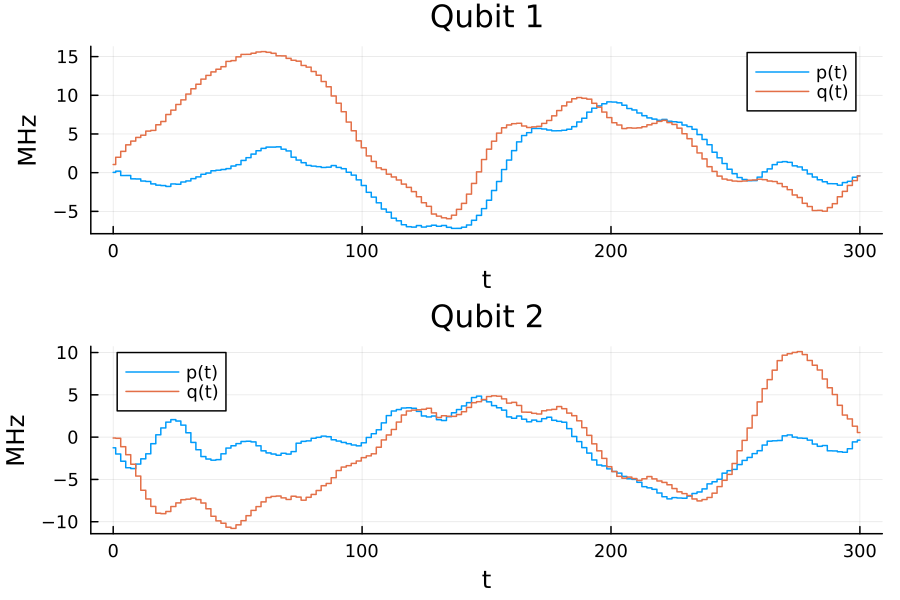
\includegraphics[width=0.65\linewidth]{images/Pulses/Pulses_plot.png}
        \caption*{}
        \label{fig:Pulses}
    \end{figure}
\end{frame}

\begin{frame}{Develop Method for continuous time Hamiltonian}
    Additionally it is valuable to develop a method that doesn't work for just pulses that aren't just piecewise-constant, for example: 
    \begin{figure}
        \centering
        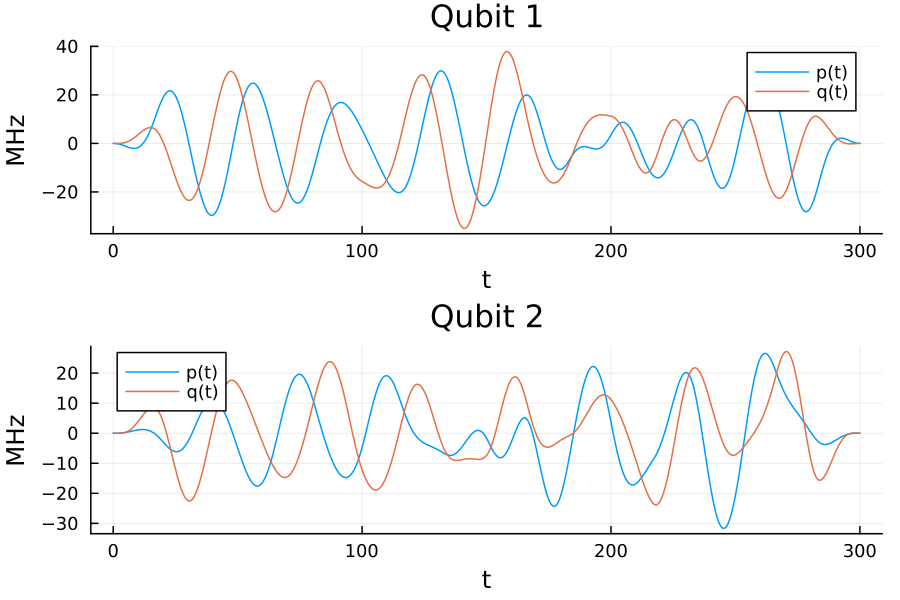
\includegraphics[width=0.8\linewidth]{images/Pulses/B_Spline_pulses_plot.png}
        \label{fig:enter-label}
    \end{figure}
\end{frame}

\begin{frame}{Continuous time Hamiltonian Method}
    Simulation using b-splines 
    \includegraphics<1>[width = 0.9\linewidth]{images/TDVP_B_Spline/TDVP1_BsplineBD4.png}
    \includegraphics<2>[width = 0.9\linewidth]{images/TDVP_B_Spline/TDVP1_BsplineBD3.png}
    \includegraphics<3>[width = 0.9\linewidth]{images/TDVP_B_Spline/TDVP1_BsplineBD2.png}
    \includegraphics<4>[width = 0.9\linewidth]{images/TDVP_B_Spline/TDVP1_BsplineBD1.png}
\end{frame}


\begin{frame}{Develop Method for Continuous time Hamiltonian}
    We can also use the TDVP2 method with this pulse, still just using an exponential solver. 
    \begin{figure}
        \centering
        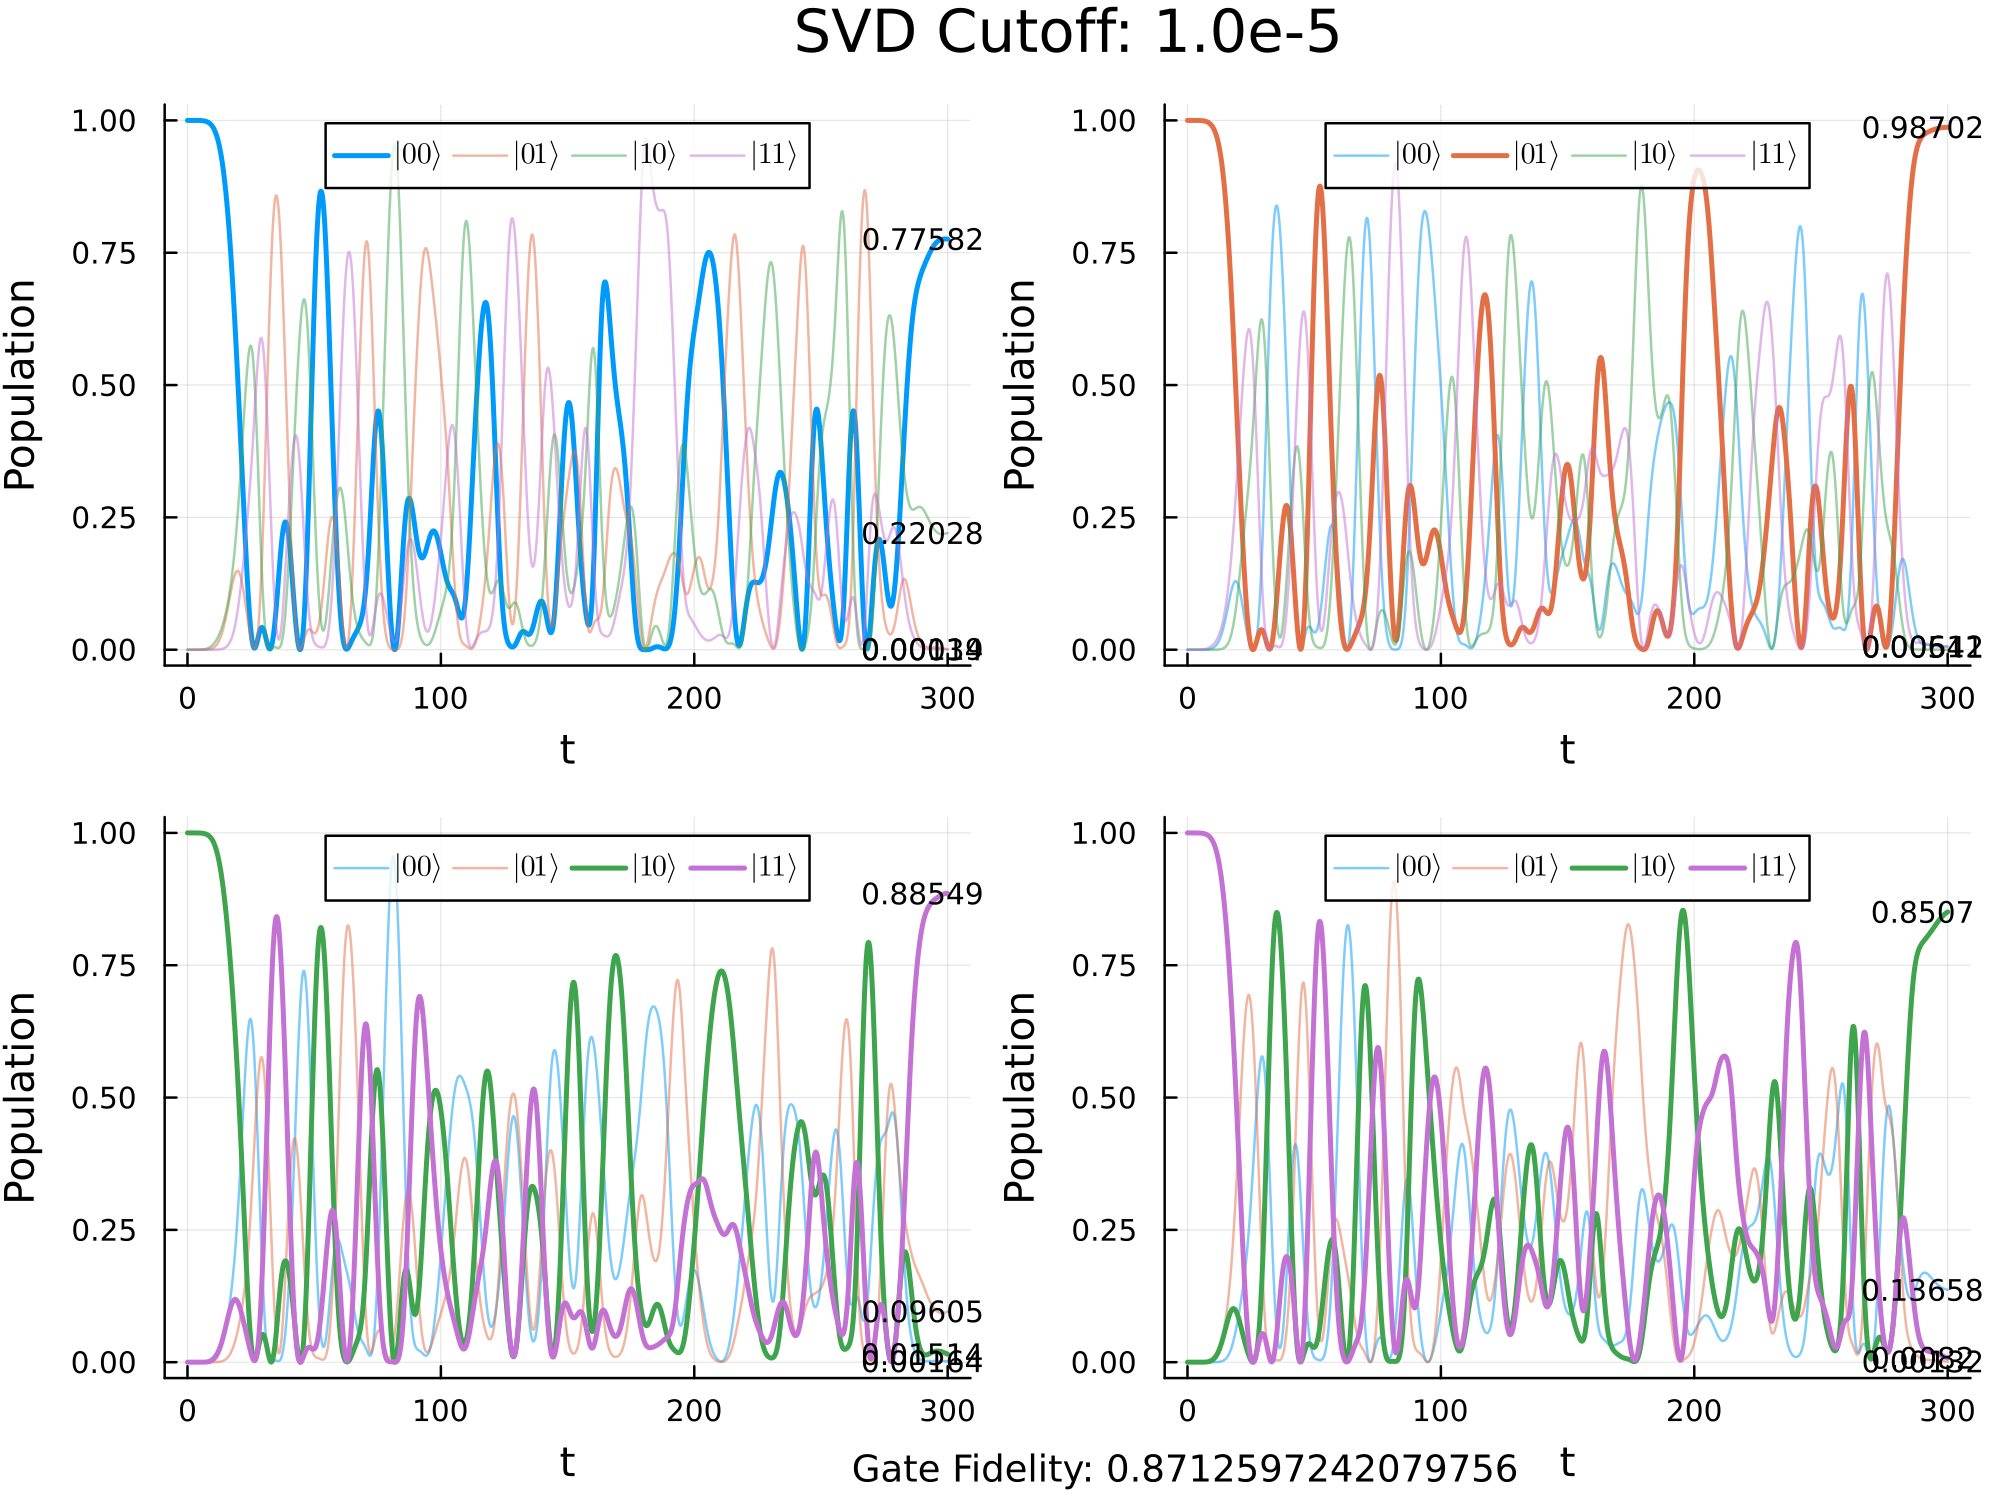
\includegraphics[width=0.9\linewidth]{images/TDVP2 Tensor Diagram/TDVP2_EvolutionSVD Cutoff_ 1.0e-5(1).png}
        \label{fig:enter-label}
    \end{figure}
\end{frame}

\begin{frame}{Combine time-evolution with Optimal Control}
    The pulses shown in previous slide were obtained from quandary.

    \begin{itemize}[<+->]
        \item Gradient Information obtained by evolving$$\begin{cases}\dot{\boldsymbol{y}} = A(t)\boldsymbol{y}\\ \, \boldsymbol{y}(0) = \boldsymbol{\eta}\end{cases},$$
    
        $$\begin{cases}
        -\dot{\boldsymbol{\lambda}} - A(t)^{\dag}\boldsymbol{\lambda} = \boldsymbol{a}(t)\\
        \boldsymbol{\lambda}(T) = \boldsymbol{w}.
        \end{cases}.$$
        \item Quandary evolves the equation using the Implicit Midpoint Rule. 
        \item For a large numbers of qubits storing vector becomes impossible. 
        \item Evolving forward using MPS can reduce the storage requirements of this evolution.
        
    \end{itemize}
\end{frame}

\begin{frame}{Beyond Dissertation}
    \begin{itemize}[<+->]
    \item Schrodinger's equation evolves a quantum state in a closed system. 
    \item An open quantum system allows for interaction with the environment.
    \item An example model of an open quantum system is the \textbf{Lindblad Master Equation},
    \begin{equation*}
        \dot{\rho} = -i(H\rho - \rho H) + \sum_{j}\gamma_jL_j\rho L_j^{\dag} - \dfrac{1}{2}\left(L_j^{\dag}L_j\rho + \rho L_j^{\dag}L_j\right)
    \end{equation*}
    \item This equation evolves a matrix $\rho$ as opposed to a vector. 
    \end{itemize}
\end{frame}

\begin{frame}[allowframebreaks]{References}
    \printbibliography
\end{frame}

\end{document}
